%%%%%%%%%%%%%%%%%%%%%%%%%%%%%%%%%%%%%%%%%%%%%%%%%%%%%%%%
% E W Fulp  2/26/2014 (CSC 790 Project 2)
%%%%%%%%%%%%%%%%%%%%%%%%%%%%%%%%%%%%%%%%%%%%%%%%%%%%%%%%
\documentclass[10pt]{article}

\usepackage[dvips]{color}
\usepackage{fancybox}
\usepackage{latexsym}
\usepackage{fancyhdr}
\usepackage{subfigure}
\usepackage{epsf}
% \usepackage{ewfcad}
% \usepackage{amsmath,amsthm}
% \usepackage{rotating}
% \usepackage{algorithmic}
% \usepackage{algorithm}
\usepackage{boxedminipage}
\usepackage{listings}
\usepackage[dvips]{color}
\usepackage{fancybox}
\usepackage{latexsym}
\usepackage{fancyhdr}
\usepackage{subfigure}
\usepackage{epstopdf}
\usepackage{slashbox}
\usepackage{amsfonts,amssymb,latexsym}
\usepackage{amsthm}  % used to make "proof" work
\usepackage{graphicx}
\usepackage{enumerate}
\usepackage{amsmath}  % added later
%\usepackage{setspace} % added later
\usepackage{color}    % added later
\everymath{\displaystyle} % added later
\usepackage{float}
\usepackage{tikz} % added later


 \textwidth=6.5in
 \oddsidemargin=0in
 \evensidemargin=0in
 \topmargin=-0.25in
 \headsep=0in
 \headheight=0in
 \textheight=9.5in

\newcommand{\window}[1]
  {
    \begin{center}
    \fcolorbox{black}{black}{\begin{minipage}{6.1in}
    \centerline{\textcolor{white}{\sf {\large $\Box$} \hfill Terminal \hfill {\large$\Box \Box$}}\vspace{0.05in}}
    \fcolorbox{white}{white}{\begin{minipage}{6.0in}
    {\tt \vspace{0.1in}#1\vspace{0.1in}}
    \end{minipage}}
    \end{minipage}}
    \end{center}
  }

\newcommand{\smallWindows}[2]
  {{ \vspace{0.125in} \footnotesize \noindent {
%     \begin{center}
    \fcolorbox{black}{black}{\begin{minipage}{3.1in}
    \centerline{\textcolor{white}{\sf {\large $\Box$} \hfill Terminal \hfill {\large$\Box \Box$}}\vspace{0.05in}}
    \fcolorbox{white}{white}{\begin{minipage}{3.0in}
    {\tt \vspace{0.1in}#1\vspace{0.1in}}
    \end{minipage}}
    \end{minipage}}
\fcolorbox{black}{black}{\begin{minipage}{3.1in}
    \centerline{\textcolor{white}{\sf {\large $\Box$} \hfill Terminal \hfill {\large$\Box \Box$}}\vspace{0.05in}}
    \fcolorbox{white}{white}{\begin{minipage}{3.0in}
    {\tt \vspace{0.1in}#2\vspace{0.1in}}
    \end{minipage}}
    \end{minipage}}

    }
   \vspace{0.125in}}
}

\newcommand{\Section}[1]{
\noindent
\hrulefill
\vspace{-0.15in}
\section{#1}
}

\newcommand{\Questions}[1]{
\subsection*{Questions {\rm \normalsize (\textsf{\textit{#1 points}})}}
}
\pagestyle{fancy}
\rhead{}\chead{}\lhead{}
\renewcommand{\headrulewidth}{0pt}
\renewcommand{\footrulewidth}{0.4pt}
\cfoot{\shortstack{\textit{\textsf{\footnotesize CSC 790}} \\
\textit{\textsf{\footnotesize Fall 2014}} \\ \thepage}}
% \lfoot{\vspace{-0.35in}\fbox{~~~~~~~~~~~~~~~~ \rule[-0.45in]{0.0in}{0.45in} }}
% \rfoot{\vspace{-0.35in}\fbox{~~~~~~~~~~~~~~~~ \rule[-0.45in]{0.0in}{0.45in} }}


\begin{document}
\newcommand{\beq}{\begin{eqnarray}}
\newcommand{\eeq}{\end{eqnarray}}

{
 \setlength{\tabcolsep}{0in}
 \noindent
 \begin{tabular*}{\textwidth}{p{4.75in}r}
 \begin{tabular}{l}
 \Large \textbf{CSC 790 A: Project 2} \\
 \Large \textbf{Landstreicher hat W\"{u}rmer gern} \\ \hline % Rainbow has Worms} \\ \hline
 \normalsize \textbf{Fall 2014}
 \end{tabular}
 &
  {\renewcommand{\arraystretch}{1.25}
  \setlength{\tabcolsep}{0.1in}
  \begin{tabular}{|l|} \hline
    \textbf{\textsf{Due}} \\ \hline \hline
    \textit{\textsf{2:00pm Thursday, 3/6}} \\ \hline
  \end{tabular}} \\ \\ \hline \hline
\end{tabular*}
}

% \vspace{-0.25in}
\section*{Project Description}

\thispagestyle{fancy}

Internet worms are a form of malware that spreads via the network
with little human assistance. The success of an Internet worm is
largely due to the ability to quickly identify vulnerable hosts.
The paper by Staniford et al.\ (reference at the course web site)
describes different methods to find vulnerable hosts, this project
will investigate the performance of these propagation methods
using simulation.


\section*{Worm Simulator}

The tar file \texttt{wormSim-2014.tar} located at the course web site
contains a simple discrete event simulator for a network of
stations (hosts). The archive consists of the five files:
\texttt{driver.cpp} contains the \texttt{main} function of the
simulator, \texttt{station.h} defines a \texttt{Station} object
that models a host, \texttt{defs.h} defines simple constants,
\texttt{event.h} defines an event in the simulator, and
\texttt{eventq.h} defines the \textit{calendar} of events.

A discrete event simulator operates by removing events from a
calendar then performing the associated task(s) for that event.
This is typically done in the \texttt{main()} function using a
\texttt{while} loop that removes the next event (which is the
current event) from the calendar then calls the correct functions
for this current event (see the \texttt{driver.cpp} file).
Therefore the calendar is modeled as an ordered (according to
time) queue of events which is defined in the \texttt{eventq.h}
file.

There are two basic events for this simulation, \texttt{Propagate}
and \texttt{Infect}. The \texttt{Propagate} event occurs when an
infected station attempts to find another vulnerable station. For
this event the \texttt{main()} will have the appropriate
\texttt{Station} object call the \texttt{propagate()} function.
This function will select another station (\textbf{you will add
the majority of your code in this function}) and insert an
\texttt{Infect} event in the calendar. The \texttt{Infect} event
causes the \texttt{infect()} function to be called. If the
\texttt{Station} associated with this call is vulnerable, then it
will insert a \texttt{Propagate} event in the calendar, which will
cause this \texttt{Station} begin infecting other stations...
\textit{and the evil continues}.

The simulator is designed to stop after all the vulnerable
stations have been infected. The simulator will continue to run
however, until all the \texttt{Events} already inserted in the
calendar have been processed. Do not change this behavior, since
the number of infection attempts will be used to compare station
selection methods.

% \subsection*{Simulator Output}

The simulator will produce 2 files per execution,
\texttt{data.dat} and \texttt{infect.dat}. The file
\texttt{data.dat} contains two columns of data, the first column
is the time (in seconds) while the second column is the number of
infected stations. The file \texttt{infect.dat} has three column:
the first column is the station index, the second column is the
time when initially infect, and the third column is the number of
infection attempts by other stations (how many times did other
stations attempt to infect this station).

\subsection*{Modeling the Network}

This project will simulate an IP class B network, which is the
same type of address space given to Wake Forest University. Class
B addresses, for example \texttt{152.17.0.0/16}, allow the last
two bytes in the IP address to be locally defined. Let's assume
this address space is subnetted where the third byte is used to
define a subnet and the fourth byte is used to define a host.
These bytes can be any value between 1 and 254. (\textit{yes there
are $2^{8}$ possible values per byte, I think 0 and 255 should be
reserved, just humor me}).

This address space can be viewed as a $254 \times 254$ matrix, for
example using the address \texttt{152.17.$x$.$y$}, the $x$ is the
row and $y$ is the column. We will assume every legal address in
the \texttt{152.17.0.0./16} has a station running, therefore there
are $254 \times 254 = 64,516$ stations in the simulator. Although
the network address space can be viewed as a matrix, it is more
easily managed in the simulator as a list (as seen in the
\texttt{driver.cpp} file). As a result we need to translate a
list index into the proper row and column index, this simple
translation in provided by the \texttt{Station} object.

\subsection*{Assumptions}

There are some important assumptions for this simulator. As
already described, it is assumed every legal address in the class
B network has a station. This results in $254 \times 254 = 64,516$
stations, but you may wish to use a smaller number for debugging
your simulator. As defined in the \texttt{main()} function,
initially only 25\% are vulnerable (you will change this value
depending on the project question).

Note, the \textbf{time in the simulator is recorded in seconds}.
There are two important random variables for the simulation, the
time to attempt an infection and the time between propagation
attempts. The time between infection is the amount of time
required for an infection attempt (for example network and
computer processing delay). For this simulation this time has a
uniform distribution between 1 and 200 milliseconds. The time
between propagation represents the time between station selection
(for example worm processing delay). For this simulation, this
time has a uniform distribution between 10 and 38 milliseconds.

% To further protect against buffer overflow attacks and other
% attacks that use shell programs, many shell programs automatically
% drop their privileges when invoked. Therefore, even if you can  ``fool''
% a privileged \setuid program to invoke a shell, you might not be able
% to retain the privileges within the shell. This protection scheme is
% implemented in {\tt /bin/bash}. In Debian, {\tt /bin/sh} is actually a
% symbolic link to {\tt /bin/bash}.  To see the life before such
% protection scheme was implemented, we  use another shell program (the
% {\tt zsh}), instead of {\tt /bin/bash}. The following instructions
% describe how to set up the {\tt zsh} program.


\Section{Random Station Selection}

For this part of the project the worm will randomly select a
station (excluding itself) within the class B address range.
Assume 25\% of the stations are vulnerable.

\Questions{10}
You must also correctly answer the following questions to receive
full credit for this part of the project.
\begin{enumerate}
  \item Describe how the worm randomly selects a
station (show your and explain your code).

  \item Plot the number of stations infected as time increases
(use hours for time). Describe the performance of the station
selection method.

  \item Plot the time until initial infection per vulnerable station. This
must be a 3 dimensional plot, where the x and y axes are the
address bytes, and the z axis is the infection time. Only
vulnerable stations should be plotted. Describe the time required
per station. Is the time the same for stations? What is the
average and standard deviation infection time? Comment on your
results.

  \item Plot the number of infection attempts per vulnerable
station. This is the number of times other stations have attempted
to infect a vulnerable station. This must be a 3 dimensional plot,
where the x and y axes are the address bytes, and the z axis is
the number of attempts. Only vulnerable stations should be
plotted. Describe the time required per station. Is the number of
infection attempts the same for stations? What is the average and
standard deviation number of  infection attempts? Comment on your
results.

   \item Change the vulnerable percentage to 50\% and repeat the
 second question. Is there a difference between the
percentages? Why or why not?
\end{enumerate}

As an example, consider a system where the maximum value of the
last two address bytes is 20. The graphs required for the first
four questions are given in figure \ref{fig:wormPerf}.

%{
%\begin{figure}
%\begin{center}
% \mbox{\centerline{{\subfigure[Number of infected stations as time increases.
%                \label{fig:infect}]
%                {{\epsfysize=1.5 in \epsffile{infect.eps}}}}
%      \quad\quad
%                   {\subfigure[Time until initial infection per vulnerable station.
%                 \label{fig:time}]
%                {{\epsfysize=1.5 in \epsffile{time.eps}}
%                }}
%\quad\quad
%                   {\subfigure[Number of infection attempts per vulnerable host.
%                 \label{fig:attempts}]
%                {{\epsfysize=1.5 in \epsffile{attempts.eps}}
%                }}                }}
%\end{center}
%\vspace{-0.15in}{\caption{An example of the three graphs required
%per experiment. This example used 20 stations per address byte.
%Note, time should be plotted in hours (not seconds as done here).
%\label{fig:wormPerf}}}
%\end{figure}

\Section{Fletcher Worm, Limited Effort Station Selection}

For this part of the project, worm will randomly select a station
(excluding itself) within the class B address range; however,
after attempting $x$ infections (does not matter if the attempt
was successful) the station will stop propagating. Assume 25\% of
the stations are vulnerable.

\Questions{15}
You must also correctly answer the following questions to receive
full credit for this part of the project.
\begin{enumerate}
  \item Describe how the worm randomly selects a station. What is
the minimum value of $x$ that will infect all vulnerable machines?

  \item Using the minimum $x$ value, plot the number of stations infected
as time increases (use hours for time). Describe the performance
of the station selection method.

  \item Using the minimum $x$ value, plot the time until initial
infection per vulnerable station (3 dimensional plot). Is the time
the same for stations? What is the average and standard deviation
infection time? Comment on your results.

  \item Using the minimum $x$ value, plot the number of infection
attempts per vulnerable station (3 dimensional plot). Describe the
time required per station. Is the number of infection attempts the
same for stations? What is the average and standard deviation
number of  infection attempts? Comment on your results.
\end{enumerate}


\Section{Topological Station Selection}

For this part of the project the worm will perform a topological
selection (excluding itself) within the class B address range. The
worm should randomly select a station within its subnet 75\% of
the time (excluding itself) and randomly select a station outside
of the local subnet 25\% of the time. Assume 25\% of the stations
are vulnerable.

\Questions{15}
You must also correctly answer the following questions to receive
full credit for this part of the project.
\begin{enumerate}
  \item Describe how the worm randomly selects a station.

  \item Plot the number of stations infected as time increases (use hours for time).
Describe the performance of the station selection method.

  \item Plot the time until initial infection per vulnerable
station (3 dimensional plot). Describe the time required per
station. Is the time the same for stations? What is the average
and standard deviation infection time? Comment on your results.

  \item Plot the number of infection attempts per vulnerable
station (3 dimensional plot). Describe the time required per
station. Is the number of infection attempts the same for
stations? What is the average and standard deviation number of
infection attempts? Comment on your results.

%   \item Change the vulnerable percentage to 50\% and repeat the
% first four questions. Is there a difference between the
% percentages? Why or why not?
\end{enumerate}

\Section{Hit List}

For this part of the project the worm will use a \textit{hit list}
that defines all hosts within the class B address range. Starting
with the first station on the list (excluding itself) the worm
should attempt to infect a station. If the infection is successful
the worm should divide its list in half, and use the first half
and instruct the newly infected station to use the second half.
Using this approach, \textbf{every station should have only one
infection attempt}. Assume 25\% of the stations are vulnerable.

\Questions{25}
You must also correctly answer the following questions to receive
full credit for this part of the project.
\begin{enumerate}
  \item Describe how the worm randomly selects a station.

  \item Plot the number of stations infected as time increases
(use hours for time). Describe the performance of the station
selection method.

  \item Plot the time until initial infection per vulnerable station
(3 dimensional plot). Describe the time required per station. Is
the time the same for stations? What is the average and standard
deviation infection time? Comment on your results.

  \item Plot the number of infection attempts per vulnerable
station (3 dimensional plot). Describe the time required per
station. Is the number of infection attempts the same for
stations? What is the average and standard deviation number of
infection attempts? Comment on your results.

%   \item Change the vulnerable percentage to 50\% and repeat
% the first four questions. Is there a difference between the
% percentages? Why or why not?
\end{enumerate}


\Section{Worm Comparison}

For this part of the project, you will compare the performance of
the previous selection methods.

\Questions{15}
You must also correctly answer the following questions to receive
full credit for this part of the project.
\begin{enumerate}
  \item Graph the number of stations infected as time increases
(use hours for time) for all the selection methods. Assume 25\% of
the stations are vulnerable. Describe the performance of the
station selection methods.  Which method is best, which is worst,
and explain why?

%   \item Would changing the vulnerable percentage to 50\% change which method was best?
%   Why or why not?

%   \item Does changing the vulnerable percentage to 50\% change
% which method is best or worst? Why or why not? How does changing
% the vulnerable percentage impact performance for all the selection
% methods?
\end{enumerate}


\Section{Worm Fight Club}

Recall the cheese worm was an attempt to make a friendly worm that would patch vulnerable systems and possibly smoke your stash (\textit{not so friendly}). This part of the project will determine if releasing a good worm that patches systems is a reasonable defense. You can assume both worms (good and bad) use identical selection methods and are released at the same time. In addition, for each station in the network identify which worm contacted it first (good or bad).

\Questions{20}

Although we all know the first rule in worm fight club, you must also correctly answer the following questions to receive
full credit for this part of the project.

\begin{enumerate}

  \item Graph the number of stations infected as time increases
(use hours for time) for all the selection methods. On the same figure also graph the number of patched systems as time increases. Assume 25\% of the stations are initially vulnerable.

  \item Run this experiment several times and record the number of infected of stations. Then create a bar chart that shows the percentage of infected hosts (x-axis) as compared to the percentage of experiments that ended with that percentage of infected hosts (y-axis). For example you may observe that 18\% of the experiments ended with 10\% of the stations infected. What is the average number of infected machines? Is this what you expected? Why or why not?
%   \item Change the vulnerable percentage to 50\% and repeat the
% first four questions. Is there a difference between the
% percentages? Why or why not?
\end{enumerate}



\section*{Solutions}
\subsection*{1.1}

In the \texttt{station.h} file, we changed the codes as follows:

\begin{lstlisting}
void propagate(double time, EventQueue& eQueue)
	{
		int toID;             // find potential victim
		int x;
		int y;
		do{
			x = rand()%MAX_STATIONS;  	// address is 152.17.x.y
			y = rand()%MAX_STATIONS;  	// address is 152.17.x.y
            		toID = x*MAX_STATIONS + y;
			}while( toID == id_ );	// selection excluding itself

    ...
    }
\end{lstlisting}
As you can see, $x$ and $y$ will be randomly assigned a value between 0 and 253, this is a 1-to-1 mapping to 1~254, besides the station vector object $s$ is also defined from 10 to $254\times254-1$, so this doesn't affect the simulation. Also, the $do...while$ loop will ensure the worm will select a station excluding itself.

\subsection*{1.2}
From \texttt{data.dat} we have
\begin{figure}[H]
\begin{center}
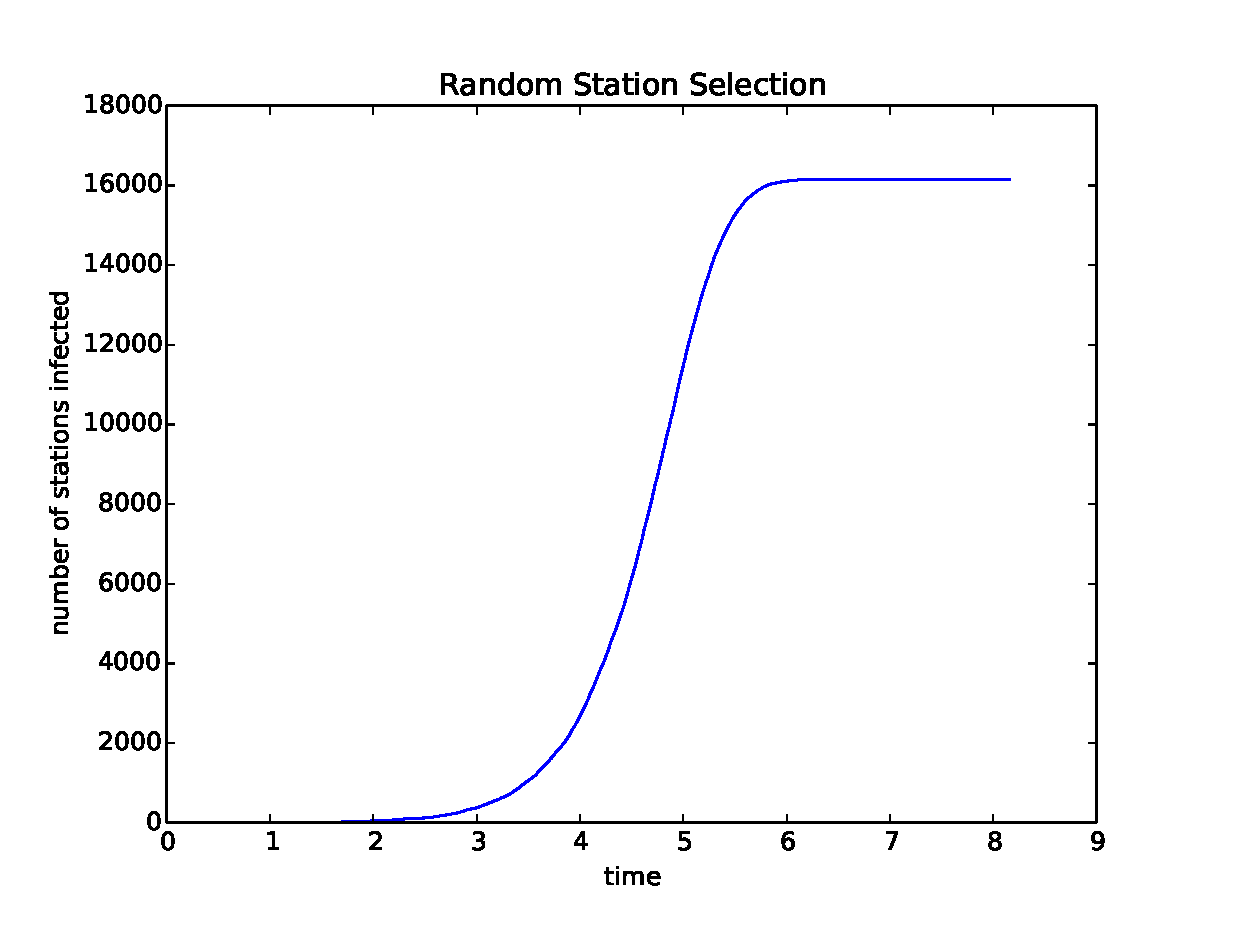
\includegraphics[width=0.8\textwidth]{figure1.2.eps}
\caption{Number of Infected Hosts using Random Station Selection}
\end{center}
\end{figure}

By the random selection method, at the beginning of propagation step, the number of infected hosts grows slower, when there are sufficient infected hosts, there is a small burst time that the number of infected hosts jumped very high, as you can that the curve is very steep in the graph.

\subsection*{1.3}
For \texttt{infect.dat} we have

\begin{figure}[H]
\begin{center}
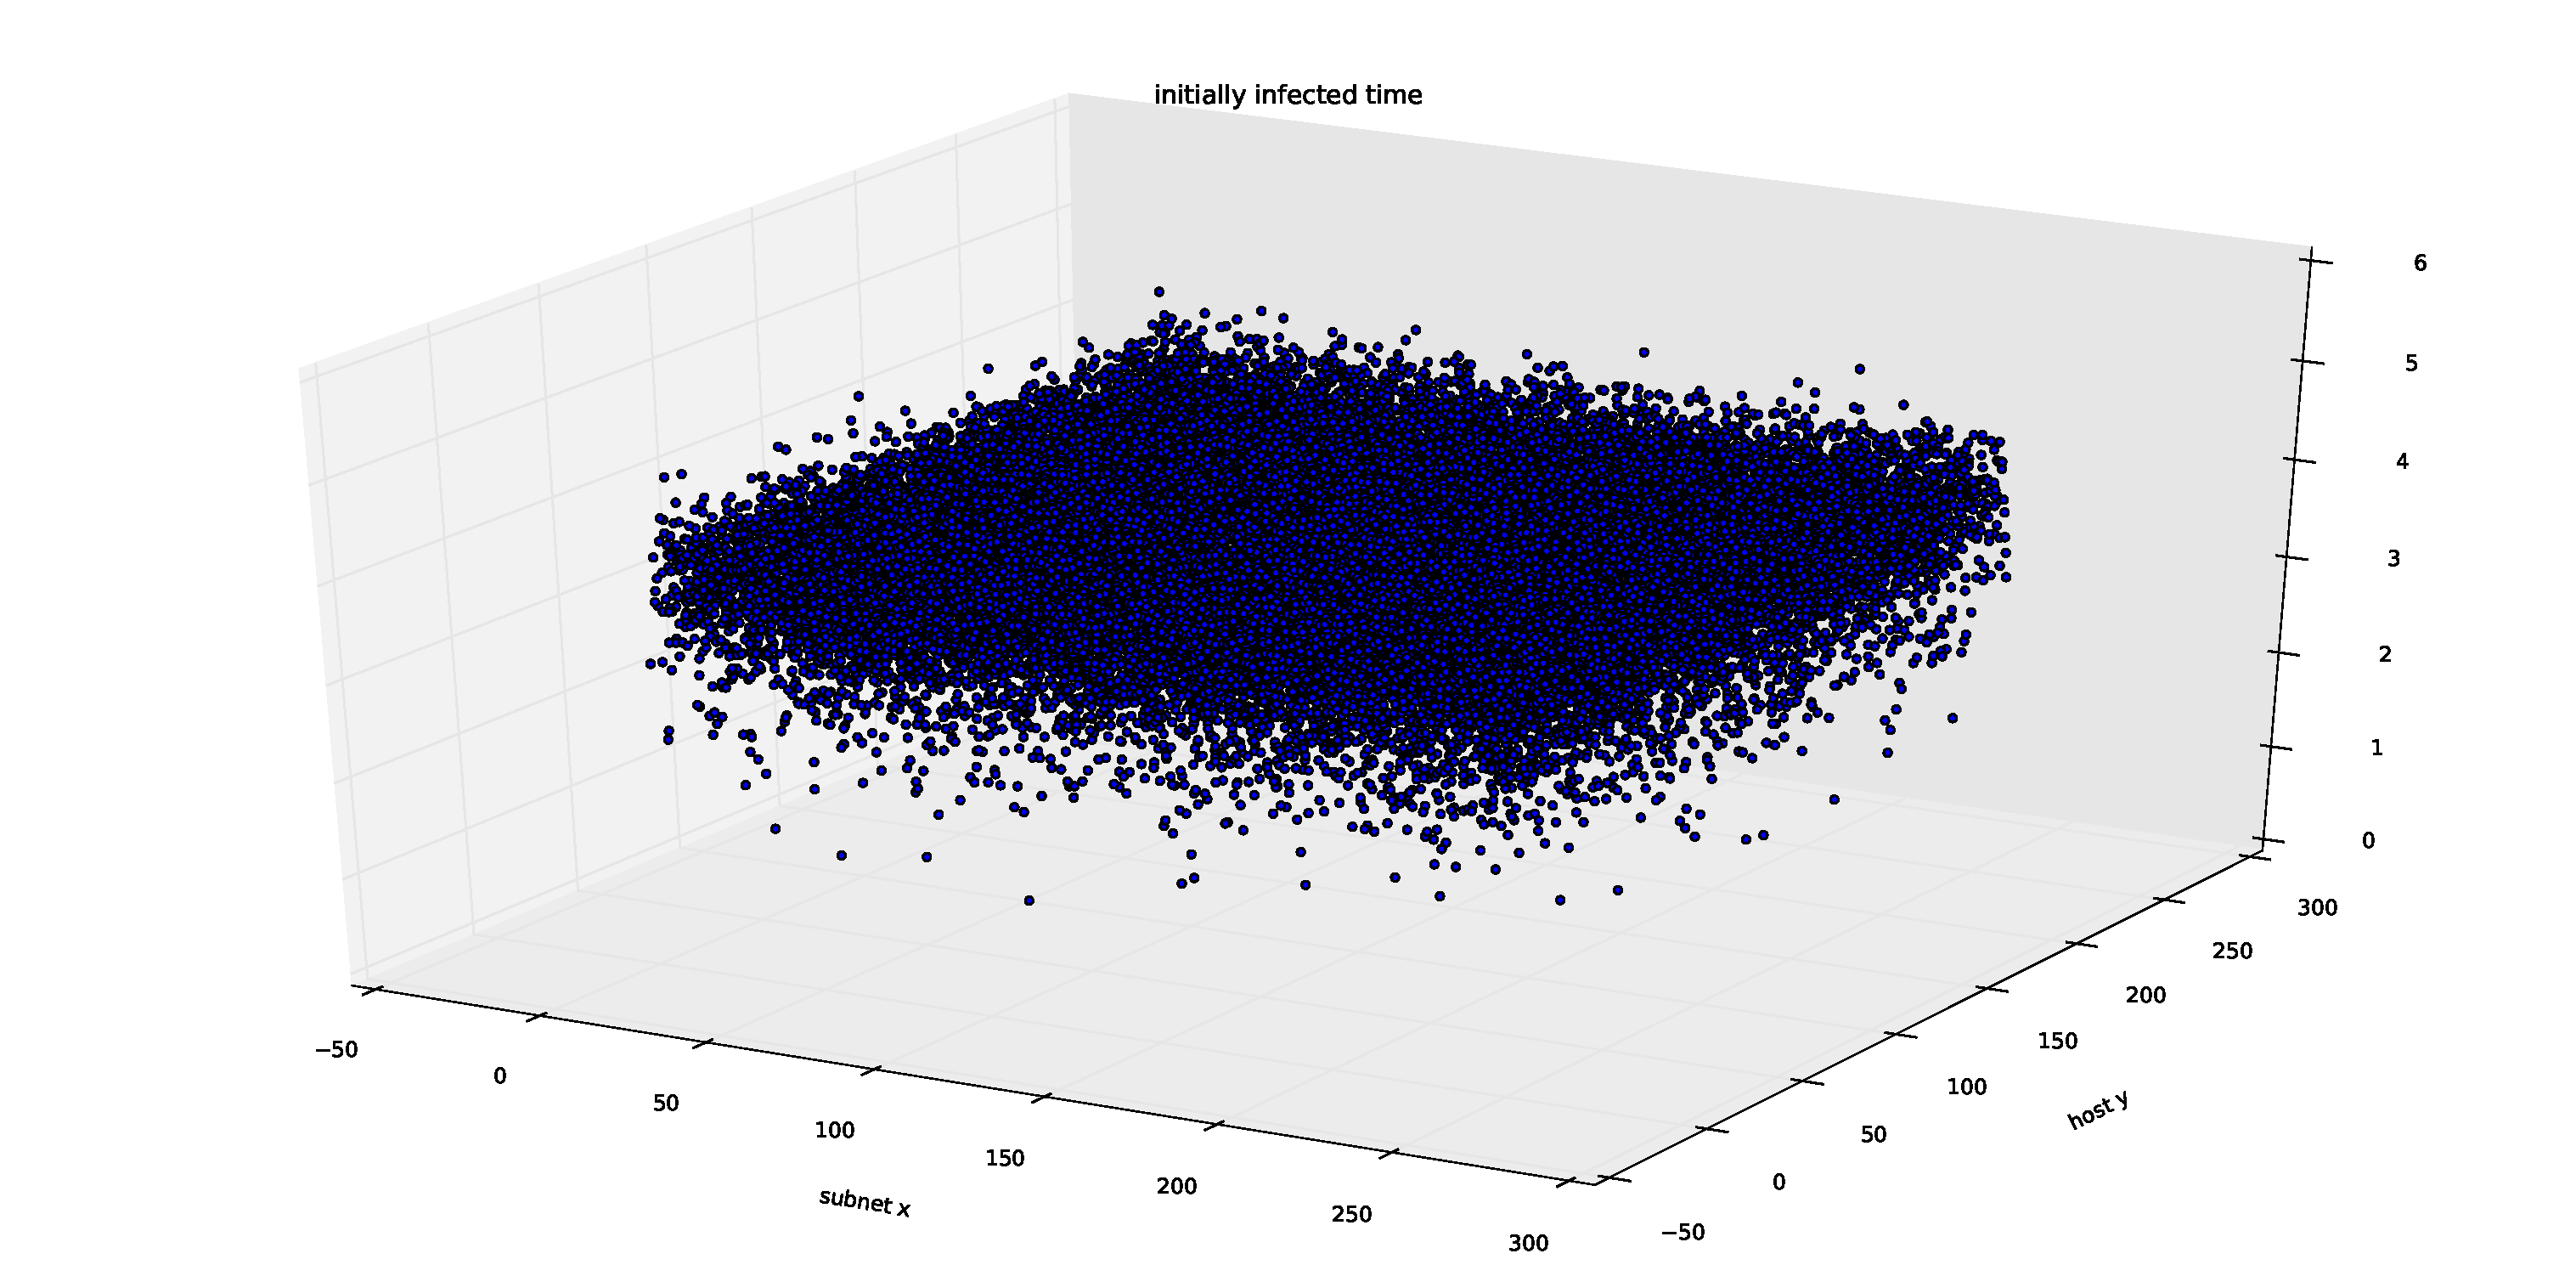
\includegraphics[width=0.8\textwidth]{figure1.3.eps}
\caption{Initially Infected Time using Random Station Selection}
\end{center}
\end{figure}

No, the time is not quite the same for stations, the average is 3.6517 and the standard deviation is 0.4951 for the infect time. Since the standard deviation is relatively small, which means most of the station get infected around almost the same time.


\subsection*{1.4}
For \texttt{infect.dat} we have

\begin{figure}[H]
\begin{center}
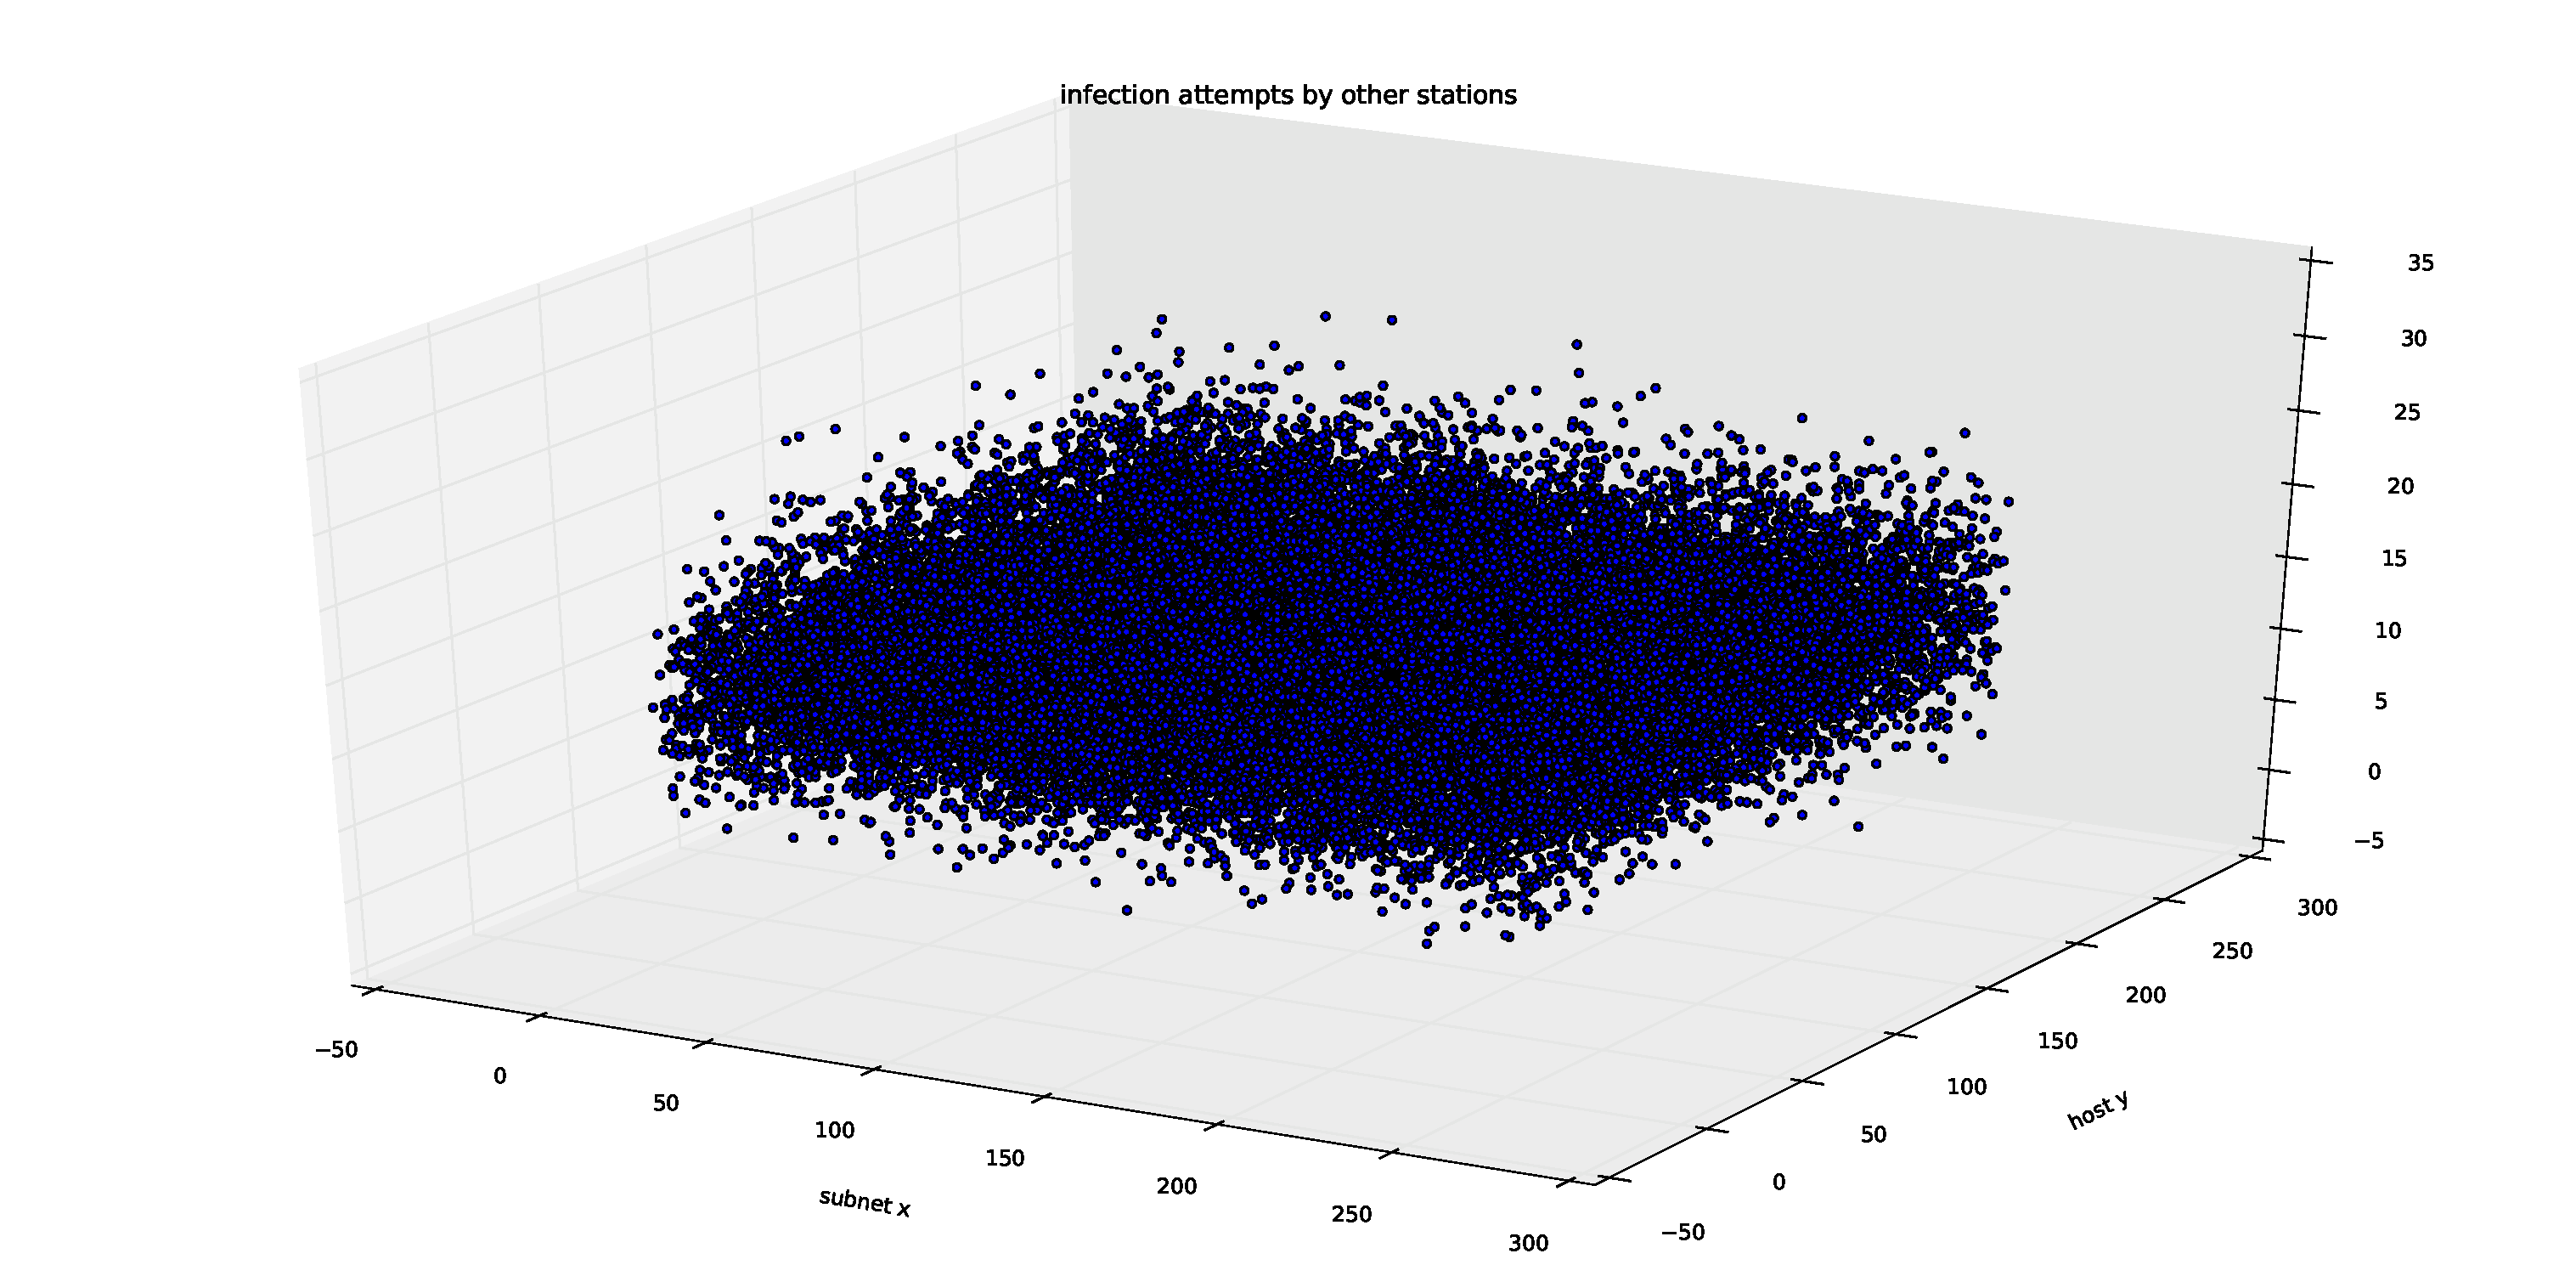
\includegraphics[width=0.8\textwidth]{figure1.4.eps}
\caption{Attempts by other Stations using Random Station Selection}
\end{center}
\end{figure}

No, the attempts is not quite the same for stations, the average is 13.23 and the standard deviation is 3.6371 for the number of the infection attempts. Here we can see that almost all vulnerable hosts got multiple infection attempts by other infected hosts.

\subsection*{1.5}
For \texttt{data.dat} we have

\begin{figure}[H]
\begin{center}
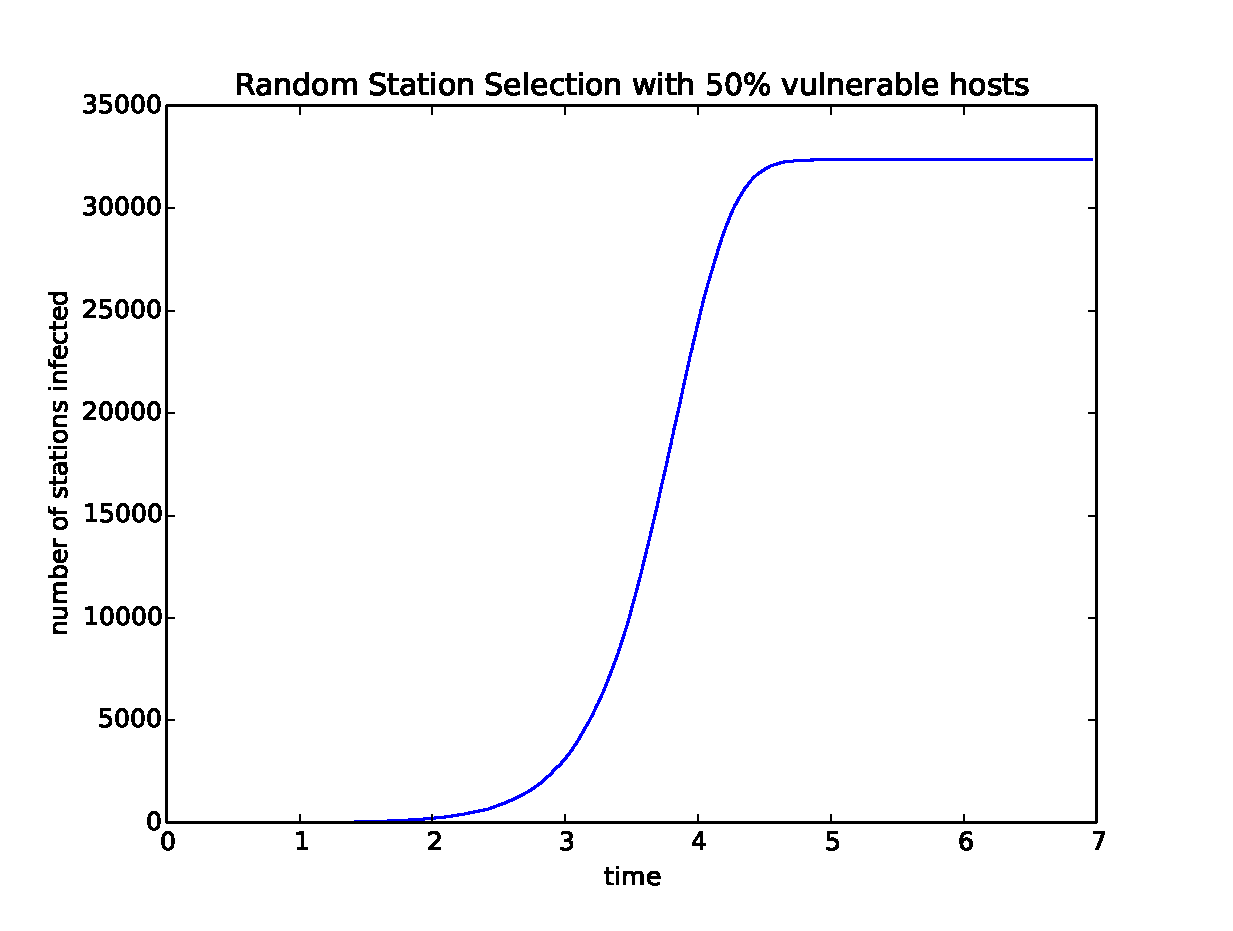
\includegraphics[width=0.8\textwidth]{figure1.5.eps}
\caption{Random Station Selection with \%50 vulnerable machines}
\end{center}
\end{figure}

Yes, clearly the number of infected hosts grow much faster when there are more vulnerable machines exists, this is more easy for worm to infect a machine and become a new source to propagate to more machines, the affect is exponentially growing.

\subsection*{2.1}

In the \texttt{station.h} file, we changed the codes as follows. The random selection method is the same with last question. After many experiments, we found that the minimum value of attempts is 36, to infect all vulnerable. We tried setting the attempts to 35 first, then number of uninfected vulnerable machines ended up with 2, then I tried 40, 37 and 36, all of them successfully infect all vulnerable machines, thus 36 is the minimum value required.
\begin{lstlisting}
class Station
{
public:
	Station(int id = 0):id_(id), vulnerable_(false), infected_(false),
		timeInfected_(0.0), numAttempt_(0), attemptUpper_(0)
	{  }
    ...
void propagate(double time, EventQueue& eQueue)
	{
		// find potential victim
		int toID;
		int x;
		int y;
		do{
			x = rand()%MAX_STATIONS;  	// address is 152.17.x.y
			y = rand()%MAX_STATIONS;  	// address is 152.17.x.y
            		toID = x*MAX_STATIONS + y;
			}while( toID == id_ );	// selection excluding itself

		if(attemptUpper_ <= 36 )
		{	
			// infect attempt time
			double infectTime = doubleUniformRV(1, 200)/1000.0;
			eQueue.insert(EventType(Infect, time + infectTime, toID, id_));

			// schedule next propagate attempt
			double interPropTime = doubleUniformRV(1, 38)/1000.0;
			eQueue.insert(EventType(Propagate, time + interPropTime, id_));
		
		attemptUpper_ ++;	
		}
    }
    ...
private:
    ...
	int     numAttempt_;     // number of infection attempts on this station
	int 	attemptUpper_;
};
\end{lstlisting}
While in the \texttt{driver.cpp} I put one extra code to see whether the
\begin{lstlisting}
bool allInfected(Station* s)
{
    ...  		
	cout 	<< "The number of vulnerable left to be infected: "
		<< numVulnerable - numInfected
		<< endl;
	return numInfected == numVulnerable;
}
\end{lstlisting}

\subsection*{2.2}
From \texttt{data.dat} we have
\begin{figure}[H]
\begin{center}
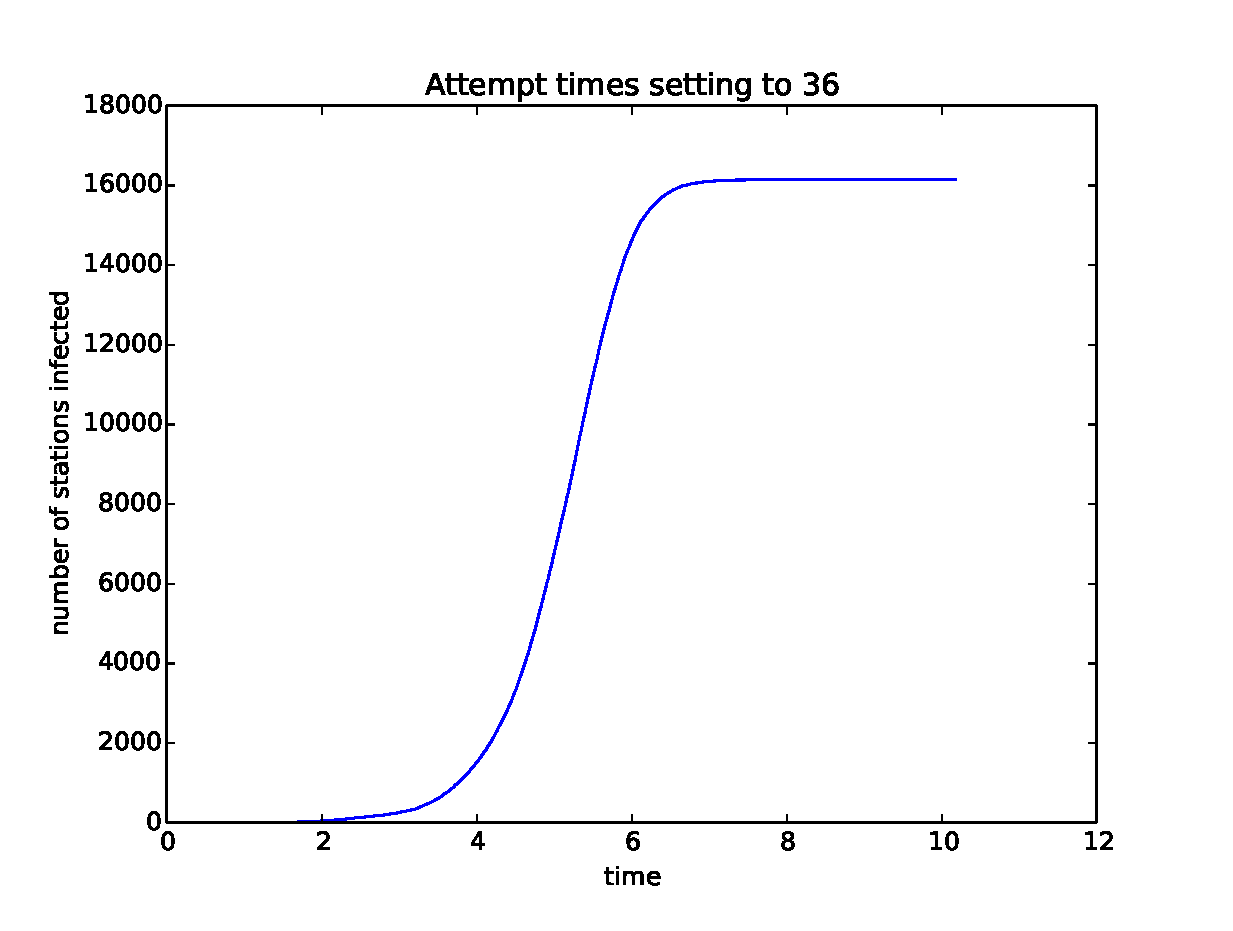
\includegraphics[width=0.8\textwidth]{figure2.2.eps}
\caption{Number of Infected Hosts using Limited Effort Station Selection}
\end{center}
\end{figure}

The performance is slightly worse than random selection method. Since the number of infection attempts are upped bounded, which compromises the abilities of the worm's propagation, even though it can accomplish the mission in the end.

\subsection*{2.3}
For \texttt{infect.dat} we have

\begin{figure}[H]
\begin{center}
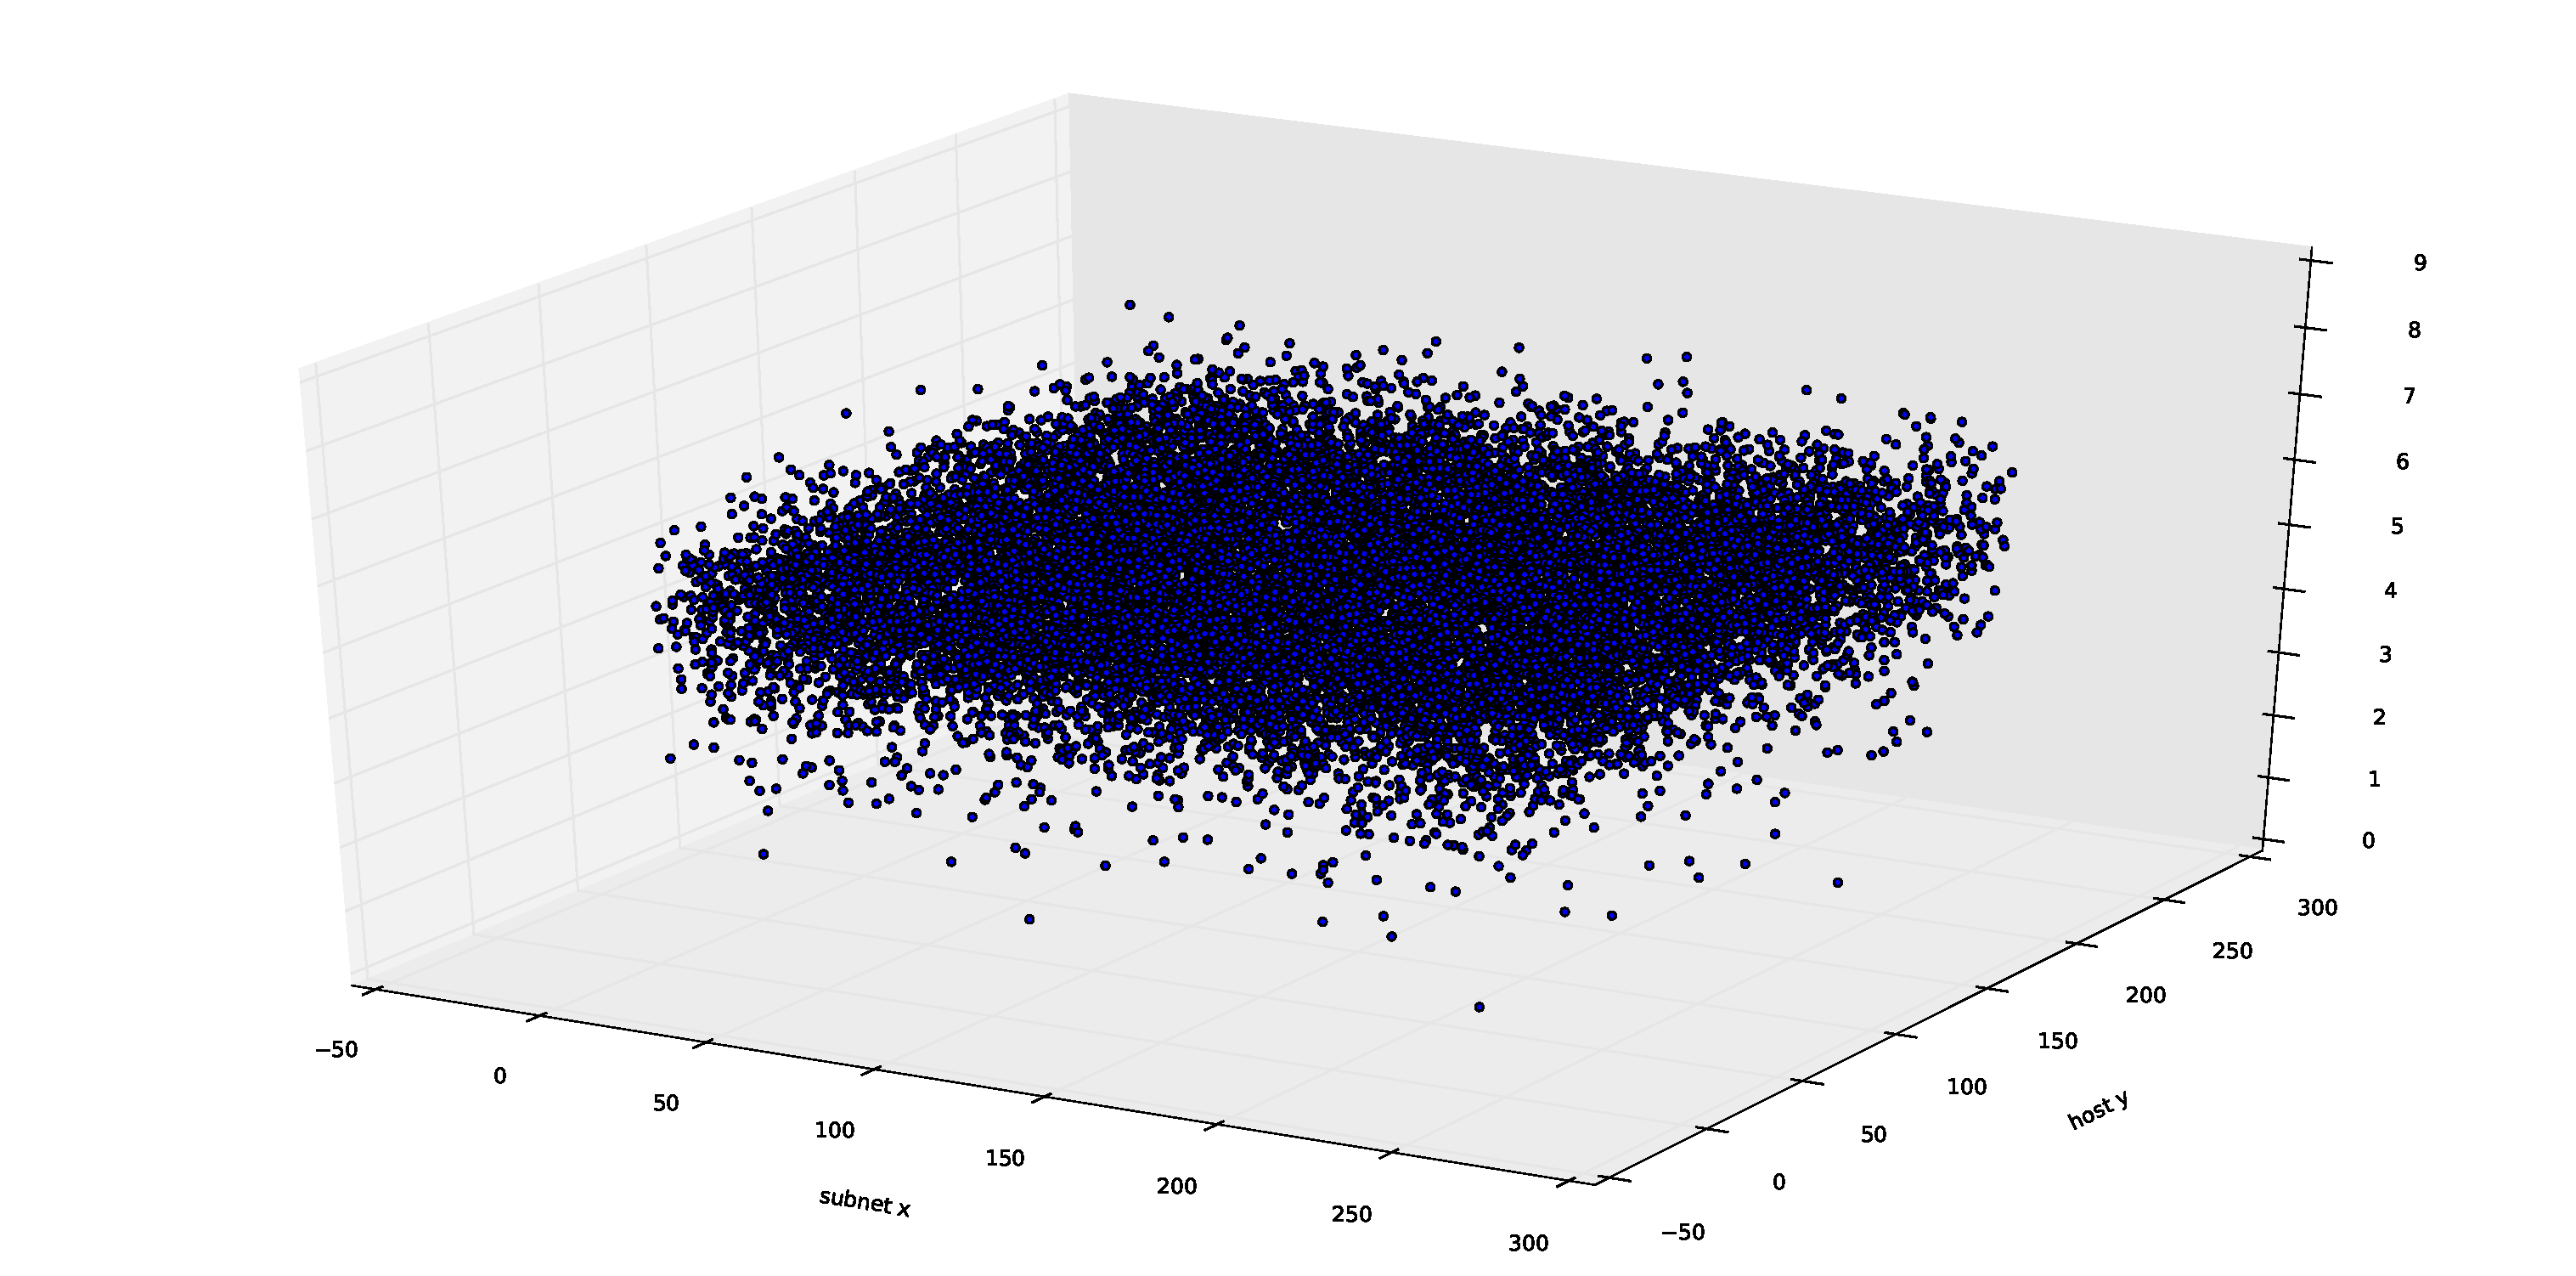
\includegraphics[width=0.8\textwidth]{figure2.3.eps}
\caption{Initially Infected Time using Limited Effort Station Selection}
\end{center}
\end{figure}

No, the time is not quite the same for stations, but very close. The average is 5.0703 and the standard deviation is 0.8005 for the infect time. As the number of attempts are bounded, thus from the standard deviation we can tell that the infect time are more centralized than random selection method, and also the average is
bigger, which means slower than the previous one.

\subsection*{2.4}
For \texttt{infect.dat} we have

\begin{figure}[H]
\begin{center}
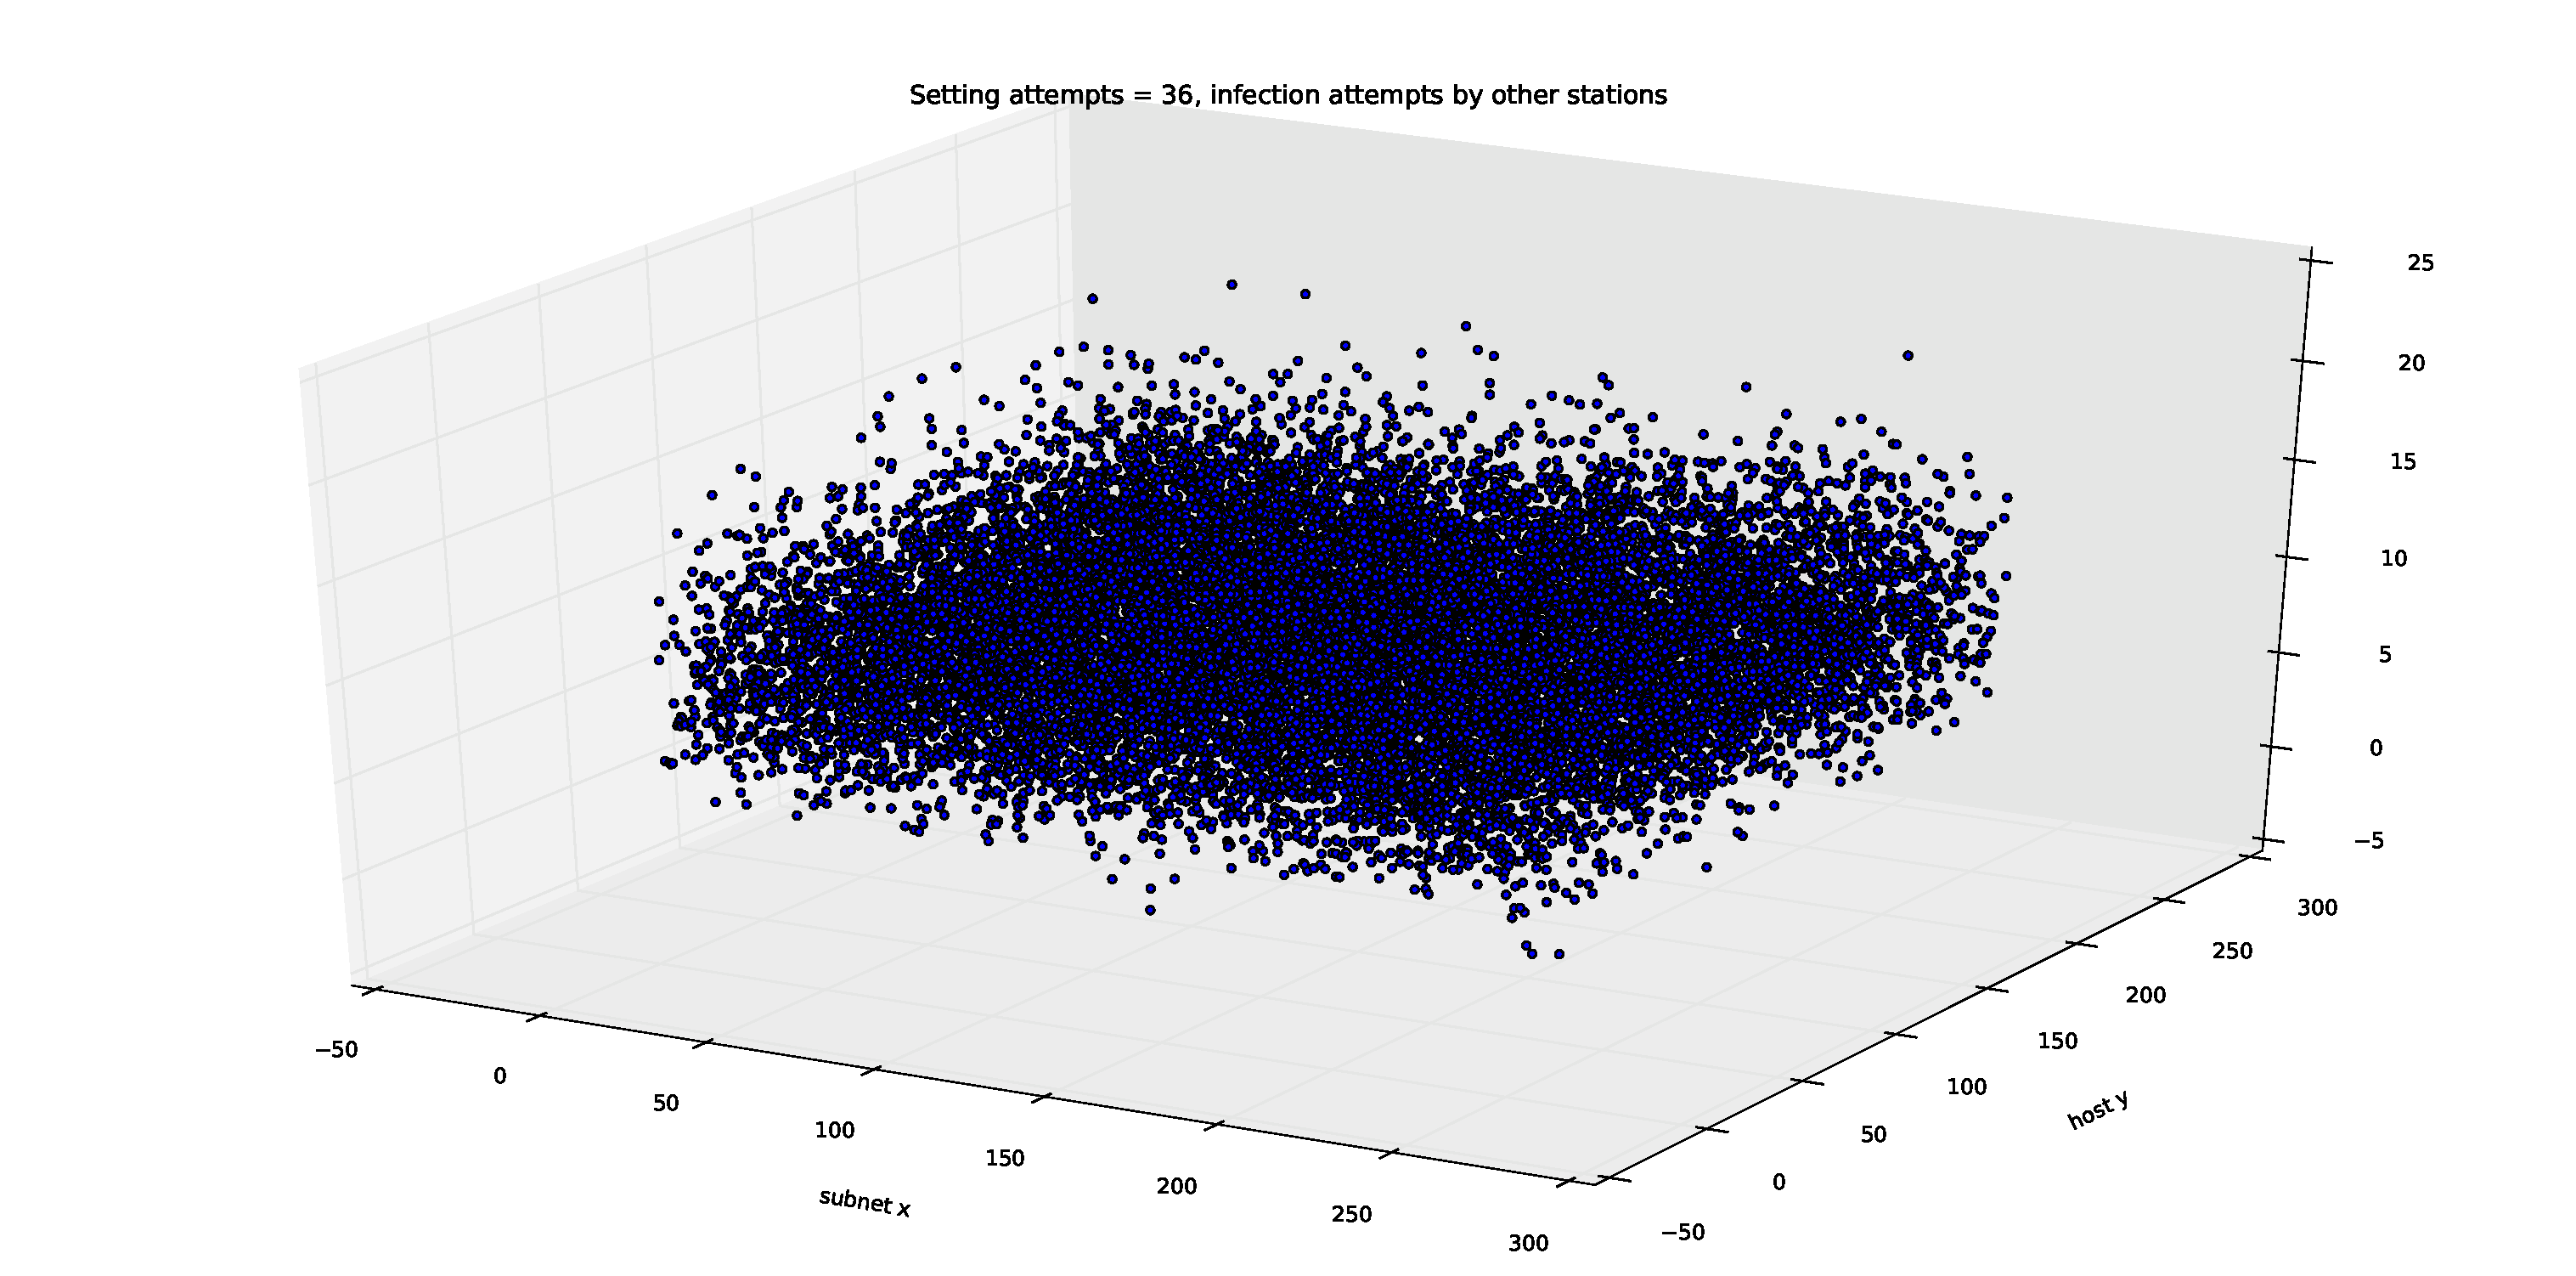
\includegraphics[width=0.8\textwidth]{figure2.4.eps}
\caption{Attempts by other Stations using Limited Effort Station Selection}
\end{center}
\end{figure}

No, the attempts is not quite the same for stations, the average is 9.0984 and the standard deviation is 3.0205 for the number of the infection attempts. As the number of attempts are bounded, we can see the average the much smaller the than random selection method, whose attempts are not bounded.

\subsection*{3.1}

In the \texttt{station.h} file, we changed the codes as follows. \%75 of the time the the subnet number is the same, other than the \%75 of the time we just randomly select number that is not the same with the local subnet number.

\begin{lstlisting}
void propagate(double time, EventQueue& eQueue)
	{
		int toID;         // find potential victim
		int x;
		int y;
		if(double(rand())/INT_MAX <= 0.75)
			x = row();	// select a station within its subnet		
		else				
			do
			{	
				x = rand()%MAX_STATIONS;  // address is 152.17.x.y
			}while( x == row() );	// select from an outside subnet	

		do
		{	
			y = rand()%MAX_STATIONS;  	// address is 152.17.x.y
			toID = x*MAX_STATIONS + y;
		}while( toID == id_ );			// selection excluding itself
    ...
    }
\end{lstlisting}


\subsection*{3.2}
From \texttt{data.dat} we have
\begin{figure}[H]
\begin{center}
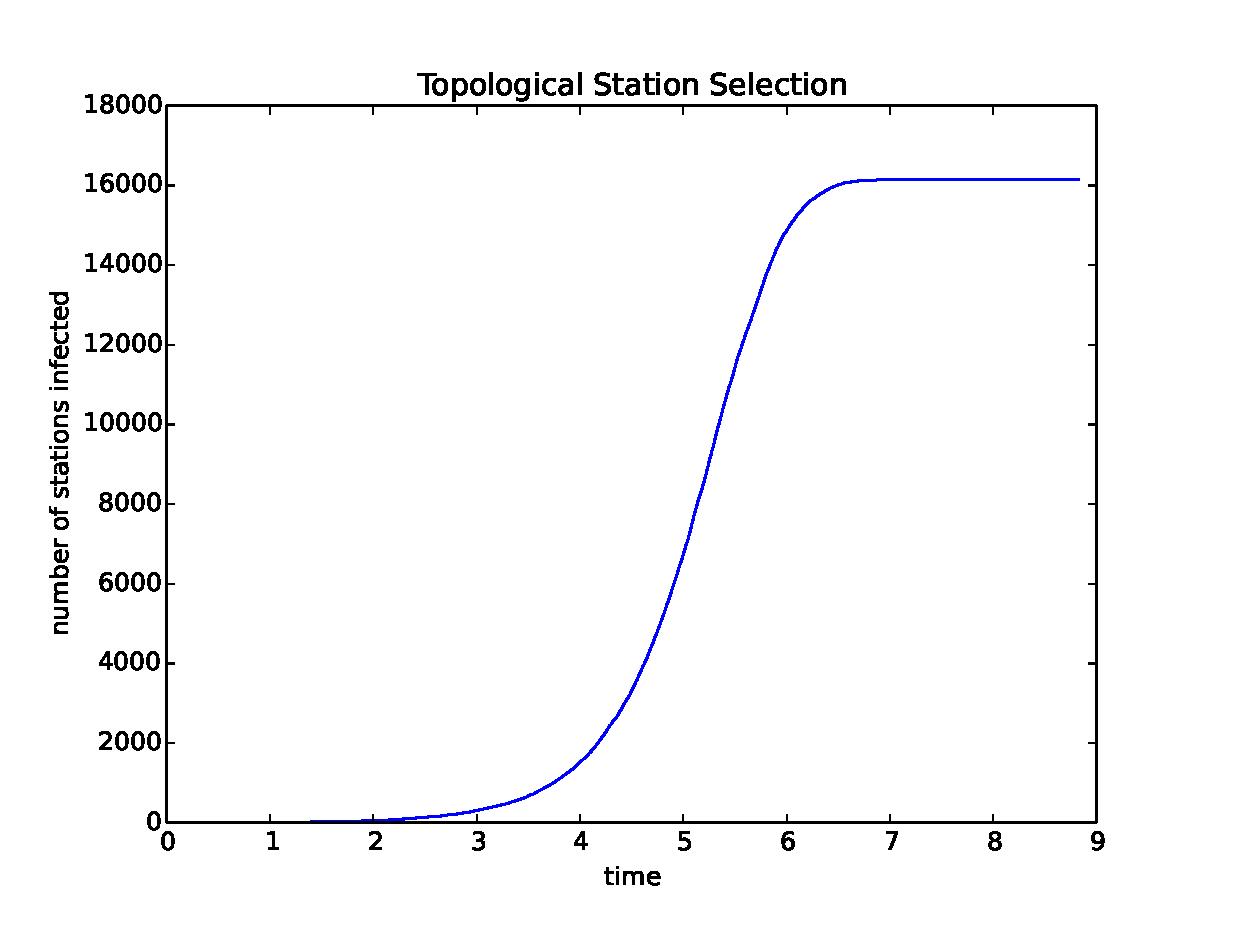
\includegraphics[width=0.8\textwidth]{figure3.2.eps}
\caption{Number of Infected Hosts using Topological Station Selection}
\end{center}
\end{figure}

The performance is very close to the random selection method, just looks like only a little bit slower.

\subsection*{3.3}
For \texttt{infect.dat} we have

\begin{figure}[H]
\begin{center}
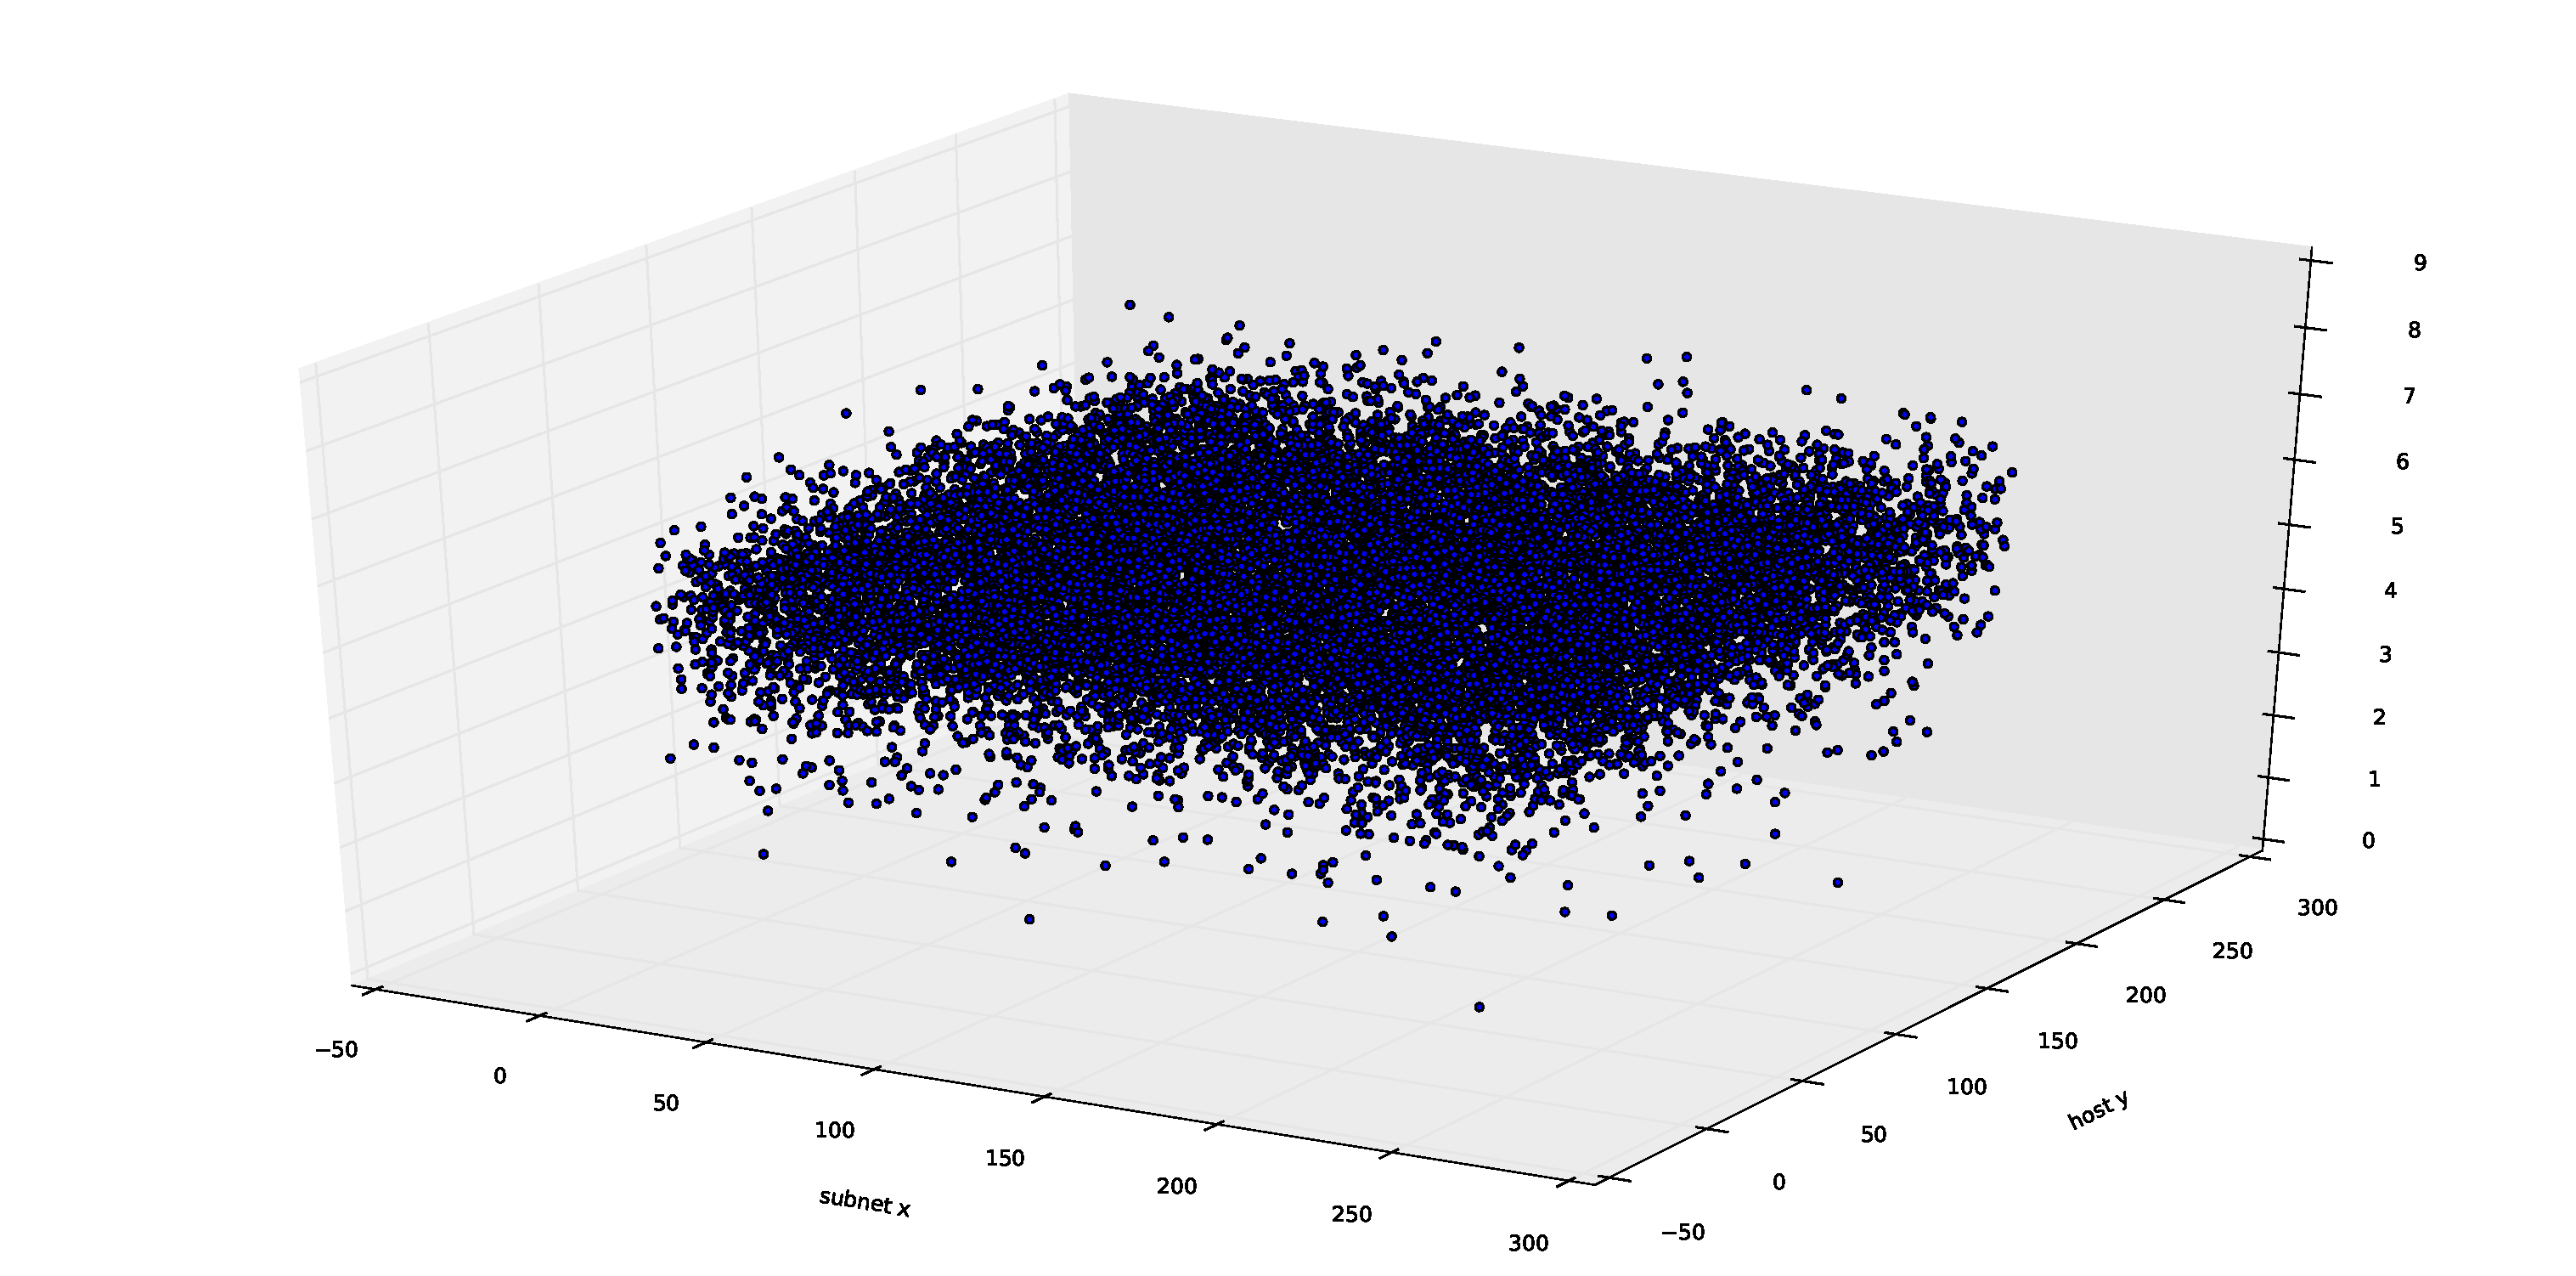
\includegraphics[width=0.8\textwidth]{figure2.3.eps}
\caption{Initial Infected Time using Topological Station Selection method}
\end{center}
\end{figure}

No, the time is not quite the same for stations, but very close. The average is 5.0451 and the standard deviation is 0.7850 for the infect time. From the standard deviation we can tell that the infect time are quite centralized than random selection method, but the average is bigger, which means slower than the previous one.

\subsection*{3.4}
For \texttt{infect.dat} we have

\begin{figure}[H]
\begin{center}
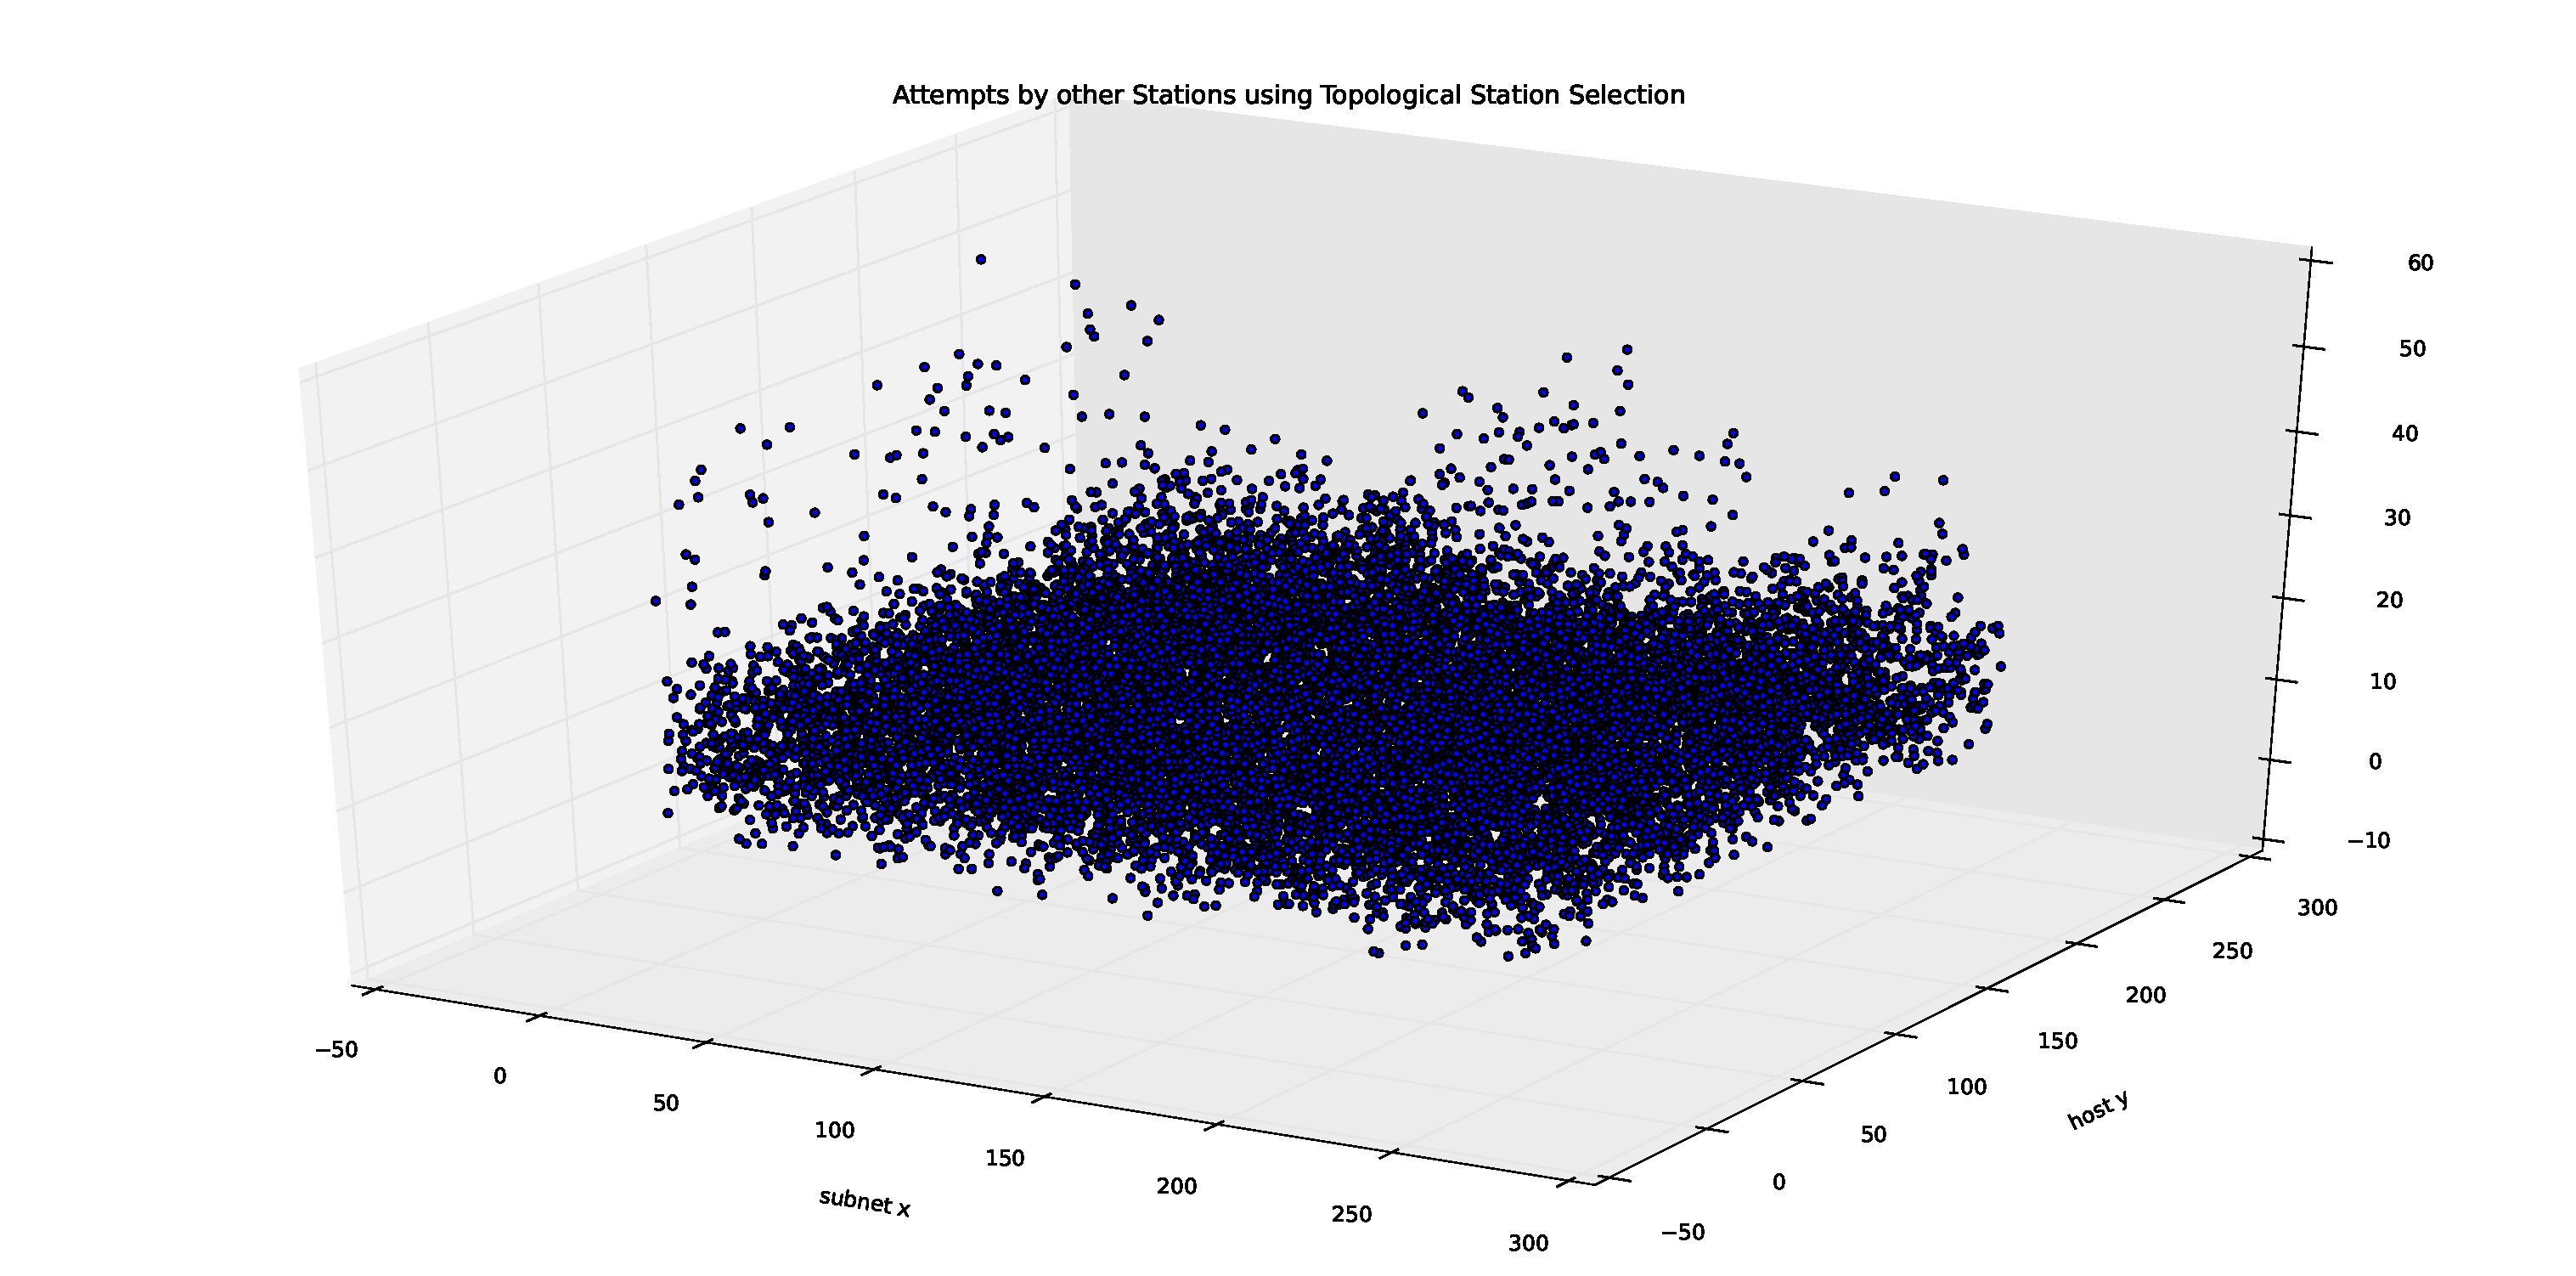
\includegraphics[width=0.8\textwidth]{figure3.4.eps}
\caption{Attempts by other Stations using Topological Station Selection}
\end{center}
\end{figure}

No, the attempts is not quite the same for stations, the average is 14.5562 and the standard deviation is 6.0005 for the number of the infection attempts. This attempts are more than the two previous ones, which indicates that the performance of worm is slightly worse when the selection are more likely to be restricted to local machines.


\subsection*{4.1}

In the \texttt{station.h} file, we assigned each station object two integers representing the beginning value and ending value of its hit list,

\begin{lstlisting}
class Station
{
public:
	Station(int id = 0):id_(id), vulnerable_(false), infected_(false),
		timeInfected_(0.0), numAttempt_(0),hit_low_(1),
        hit_up_(MAX_STATIONS*MAX_STATIONS-1)
	{  }
	
	void setLow(int low)
	{  hit_low_ = low;  }
	void setUp(int up)
	{  hit_up_ = up;   }
	int getLow()
	{  return hit_low_;}
	int getUp()
	{  return hit_up_;}
    ...

private:
    ...
	int 	hit_low_;	// begin value of the hit list
	int 	hit_up_;	// end value of the hit list
};
\end{lstlisting}

We also modified the \texttt{propagate()} and \texttt{propagate()} function such that after each successful infection, their hit list will be halved and continue to propagate with the first half, while the infected host will use the second half of the hit list.

\begin{lstlisting}
	void propagate(double time, EventQueue& eQueue, Station* s)
	{
		int toID;	// find potential victim
		if ( hit_low_ <= hit_up_ )
		{
			do
			{
				toID = hit_low_;
				hit_low_ ++;
			}while( id_ == toID );

			// infect attempt time
			double infectTime = doubleUniformRV(1, 200)/1000.0;
			eQueue.insert(EventType(Infect, time + infectTime, toID, id_));

			// schedule next propagate attempt
			double interPropTime = doubleUniformRV(1, 38)/1000.0;
			eQueue.insert(EventType(Propagate, time + interPropTime, id_));
		}
	}

	void infect(double time, EventQueue& eQueue, Station* s , int fromID)
	{
		numAttempt_++;  // someone attempts to infect, add to count
		if(vulnerable_ && !infected_)
		{	
			if( id_ > 0)
			{	
				int fromID_low = s[fromID].getLow();
				int fromID_up = s[fromID].getUp();
				setLow( (fromID_low + fromID_up)/2+1);
				setUp(fromID_up);
				s[fromID].setUp( (fromID_low + fromID_up)/2 );
			}
			infected_ = true;
			timeInfected_ = time;
			// schedule next propagate attempt
			double interPropTime = doubleUniformRV(1, 20)/10.0;
			eQueue.insert(EventType(Propagate, time + interPropTime,id_ ));
		}
	}
\end{lstlisting}

So, we also modified the \texttt{main()} function in the  \texttt{driver.app} accordingly.
\begin{lstlisting}
while(!eventQueue.isEmpty())
	{
    ...
		switch(currentEvent.event())
		{
			//--Propagate--------------------------------------------
			case Propagate:
				if(!allInfected(s))
					s[toID].propagate(time, eventQueue, s);
				break;
			//--Infect-----------------------------------------------
			case Infect:
				
				s[toID].infect(time, eventQueue, s, fromID);
				break;
			//--illegal event----------------------------------------
			default:
				cout << "Illegal event \n";
				cout << "http://goo.gl/QMET";
		}
    ...
\end{lstlisting}

\subsection*{4.2}

From \texttt{data.dat} we have
\begin{figure}[H]
\begin{center}
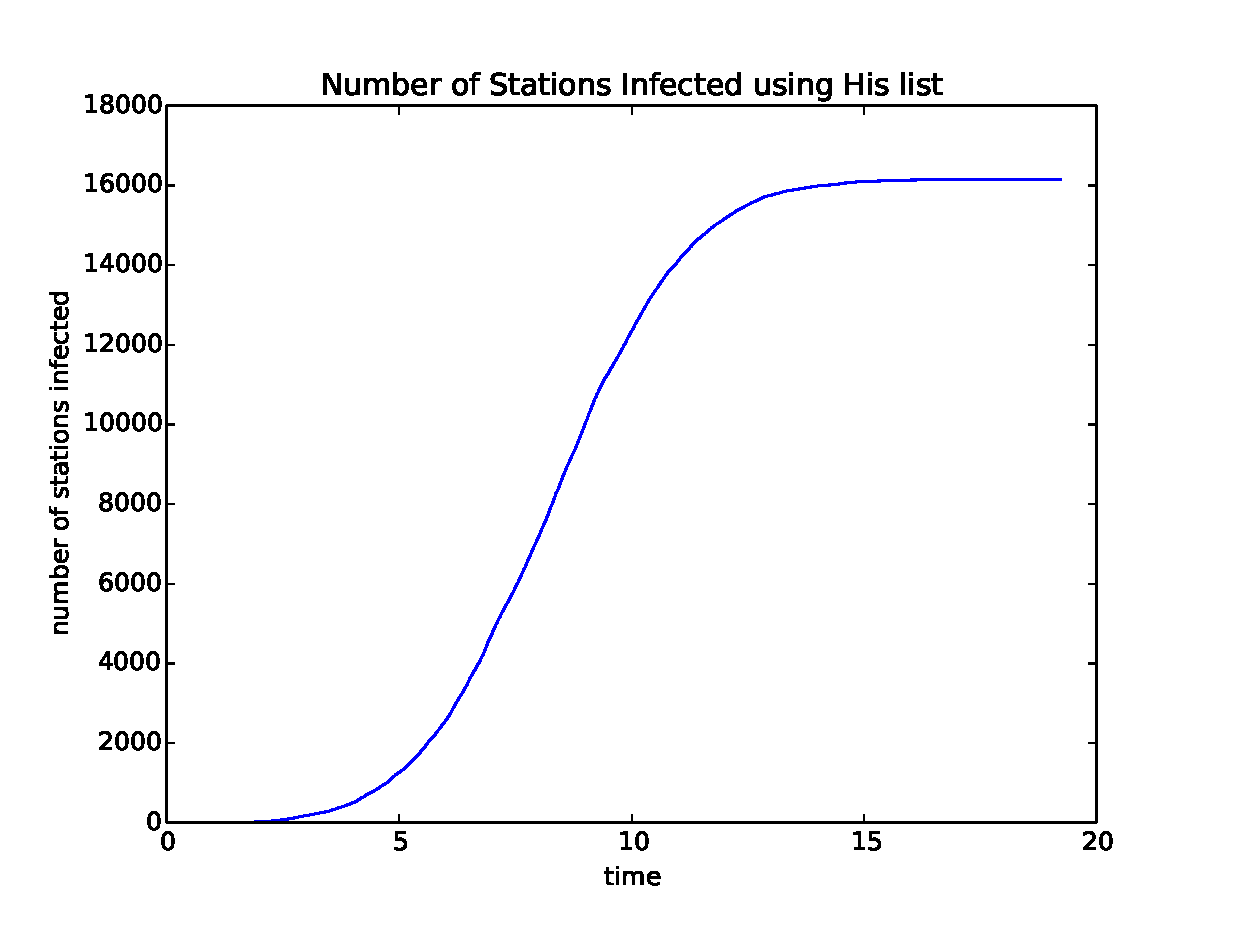
\includegraphics[width=0.8\textwidth]{figure4.2.eps}
\caption{Number of Infected Hosts using Hit List}
\end{center}
\end{figure}

The performance much worse than either the random selection method or topological station selection method. Since the hit list is more like linear search, it takes longer time to find the second vulnerable machine than randomly selection, thus the burst period came later than randomly selection method.

\subsection*{4.3}
For \texttt{infect.dat} we have

\begin{figure}[H]
\begin{center}
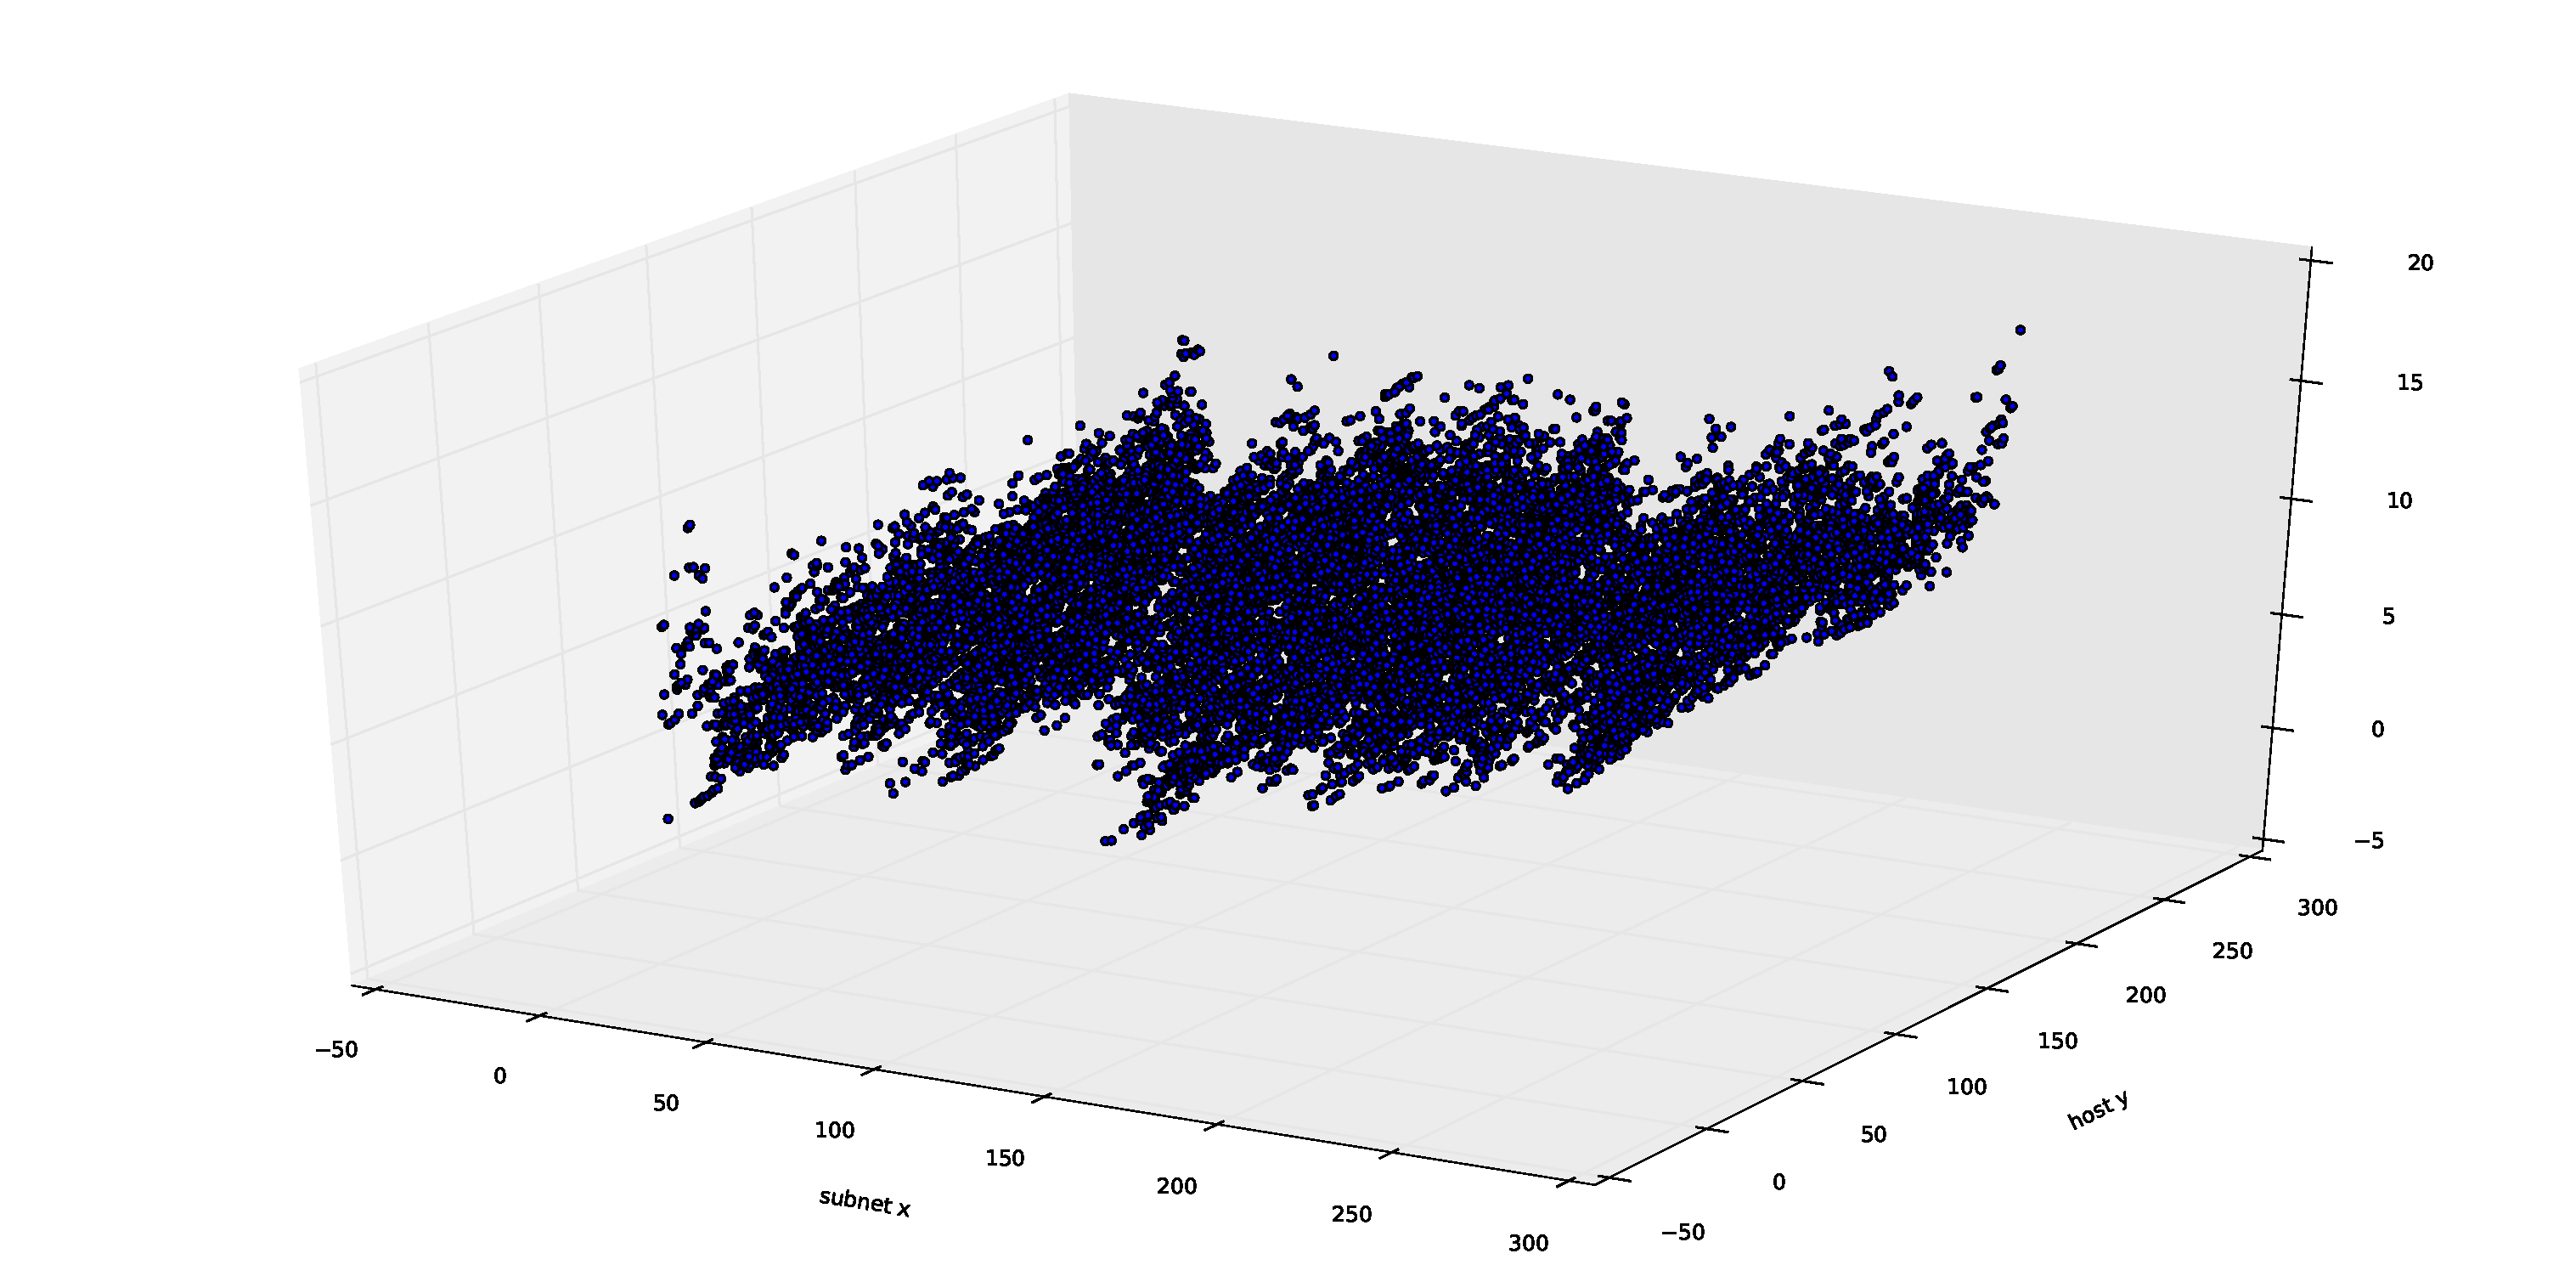
\includegraphics[width=0.8\textwidth]{figure4.3.eps}
\caption{Initial Infected Time using His list}
\end{center}
\end{figure}

No, the time is not the same for stations. The average is 8.3191 and the standard deviation is 2.3487 for the infect time. As we can see here that it takes longer to infect all the vulnerable machines. Since the worm attempt to infect from smaller station ID to bigger ones on the hit list, thus the vulnerable machines with larger station ID are infected at the very end.

\subsection*{4.4}
For \texttt{infect.dat} we have

\begin{figure}[H]
\begin{center}
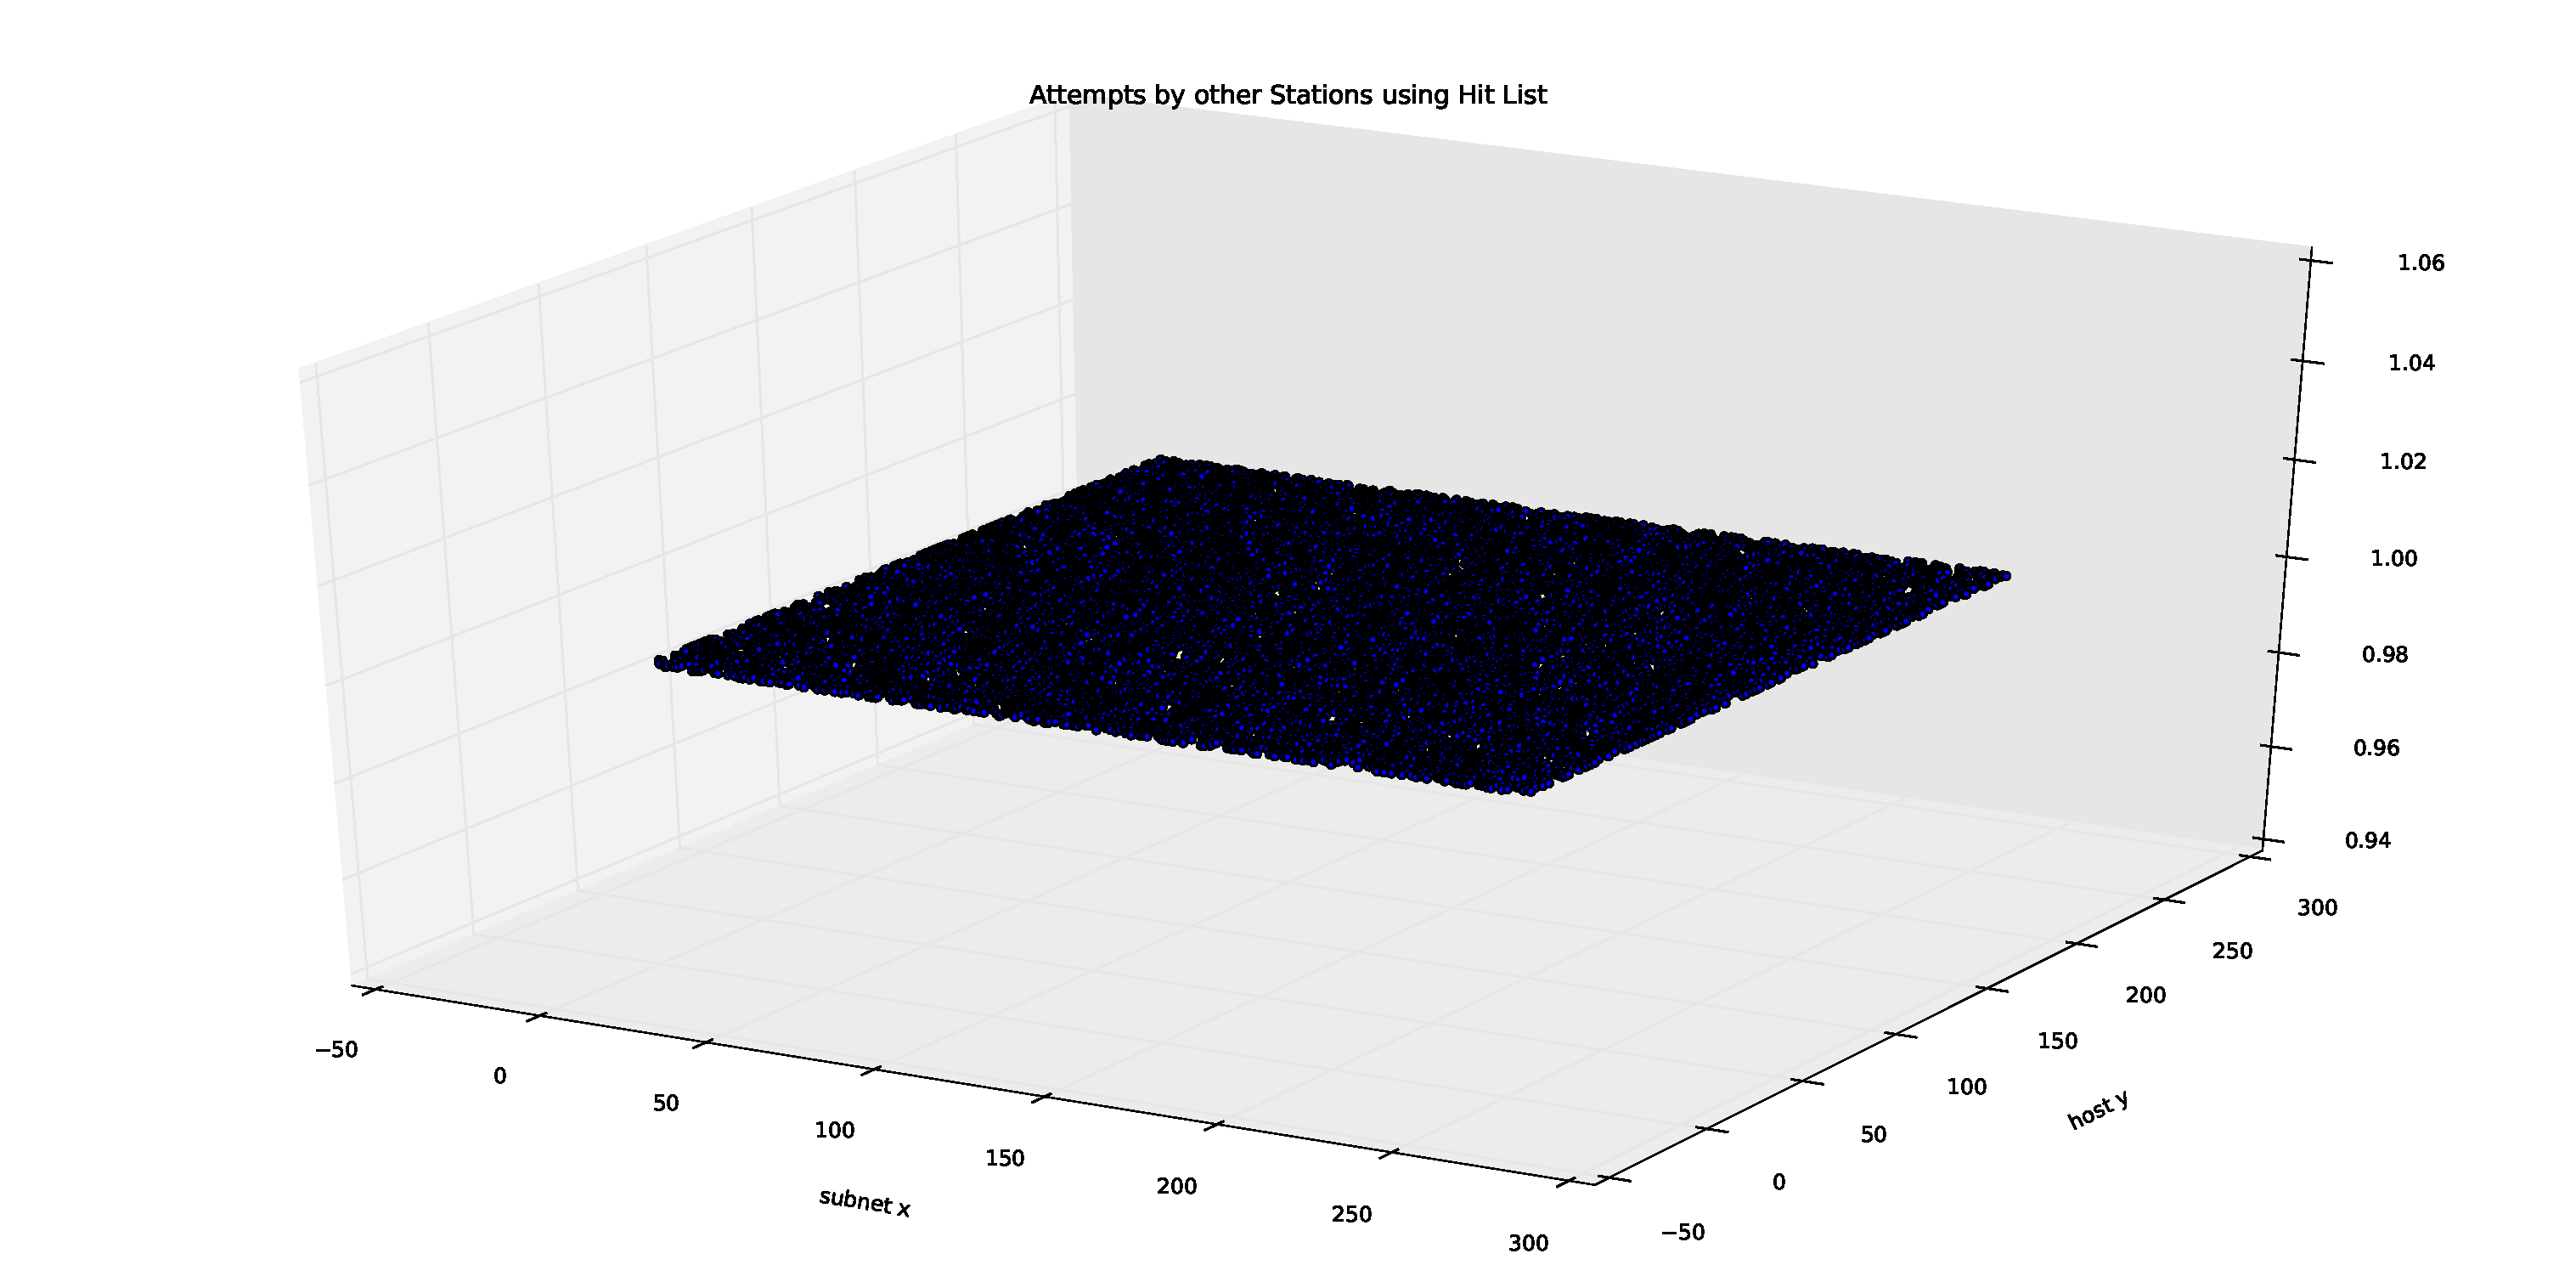
\includegraphics[width=0.8\textwidth]{figure4.4.eps}
\caption{Attempts by other Stations using Hit List}
\end{center}
\end{figure}

Yes, the attempt times are exactly the same for all the stations, the average is 1 and the standard deviation is 0. This because worm is using the hit list, and will try to infect each station exactly once.


\subsection*{5.1}

From each \texttt{data.dat} file we have above for each method, we have

\begin{figure}[H]
\begin{center}
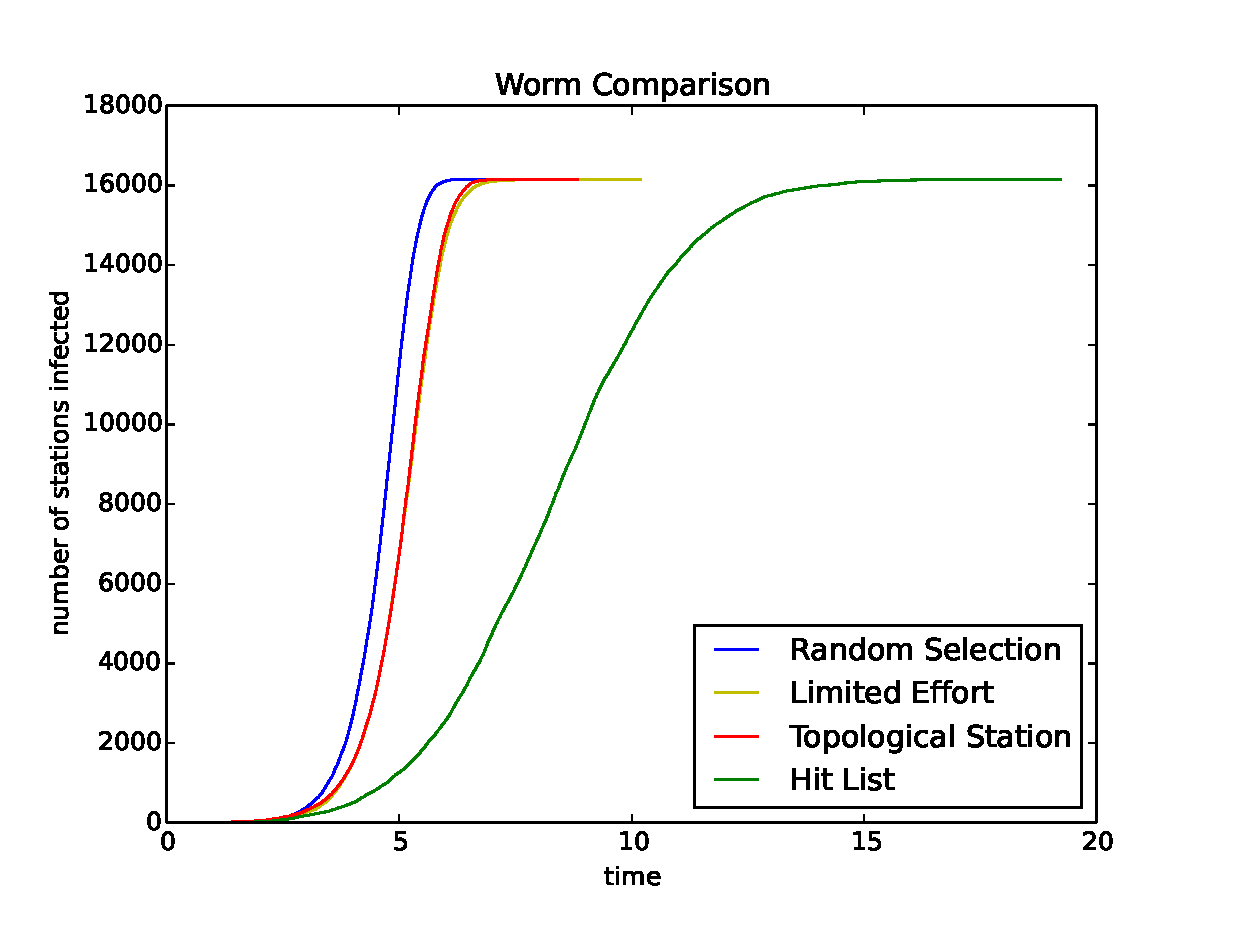
\includegraphics[width=0.8\textwidth]{figure5.1.eps}
\caption{Worm Comparison in Number of Infected hosts over Time}
\end{center}
\end{figure}

As can see from the figure above, that the random selection method is the best in terms of worm propagation, Limited Effort method and Topological Station Selection method are very close to each other, and using hit list will cost the most time and infect all vulnerable machines.


\subsection*{6.1}
Now I am using random selection as an example, to show what I changed on the codes.

In the \texttt{event.h} file, we added two more events:
\begin{lstlisting}
...
enum Event{Infect, Propagate_Infect, Secure, Propagate_Secure};
...
\end{lstlisting}

In the \texttt{station.h}, we added two more functions \texttt{propagate\_secure} and \texttt{secure}. 

\begin{lstlisting}
...
void propagate_secure(double time, EventQueue& eQueue)
	{
		// find potential victim
		int toID_s;
		int x_s;
		int y_s;
		do
		{
			x_s = rand()%MAX_STATIONS;;  // address is 152.17.x.y
			y_s = rand()%MAX_STATIONS;;  // address is 152.17.x.y
			toID_s = x_s * MAX_STATIONS + y_s;
		}while( toID_s == id_ );
		// infect attempt time
		double secureTime = doubleUniformRV(1, 200)/1000.0;  
		eQueue.insert(EventType(Secure, time + secureTime, toID_s, id_));

		// schedule next propagate attempt
		double interPropTime = doubleUniformRV(1, 38)/1000.0;
		eQueue.insert(EventType(Propagate_Secure, time + interPropTime, id_));
	}

void secure(double time, EventQueue& eQueue)
	{
		if(vulnerable_ && !infected_)
		{
			vulnerable_ = false;
			//infected_ = true;
			timeInfected_ = time;
			// schedule next propagate attempt
			double interPropTime = doubleUniformRV(1, 20)/10.0;
			eQueue.insert(EventType(Propagate_Secure,time+interPropTime,id_));
		}
	}
...
\end{lstlisting}

In the \texttt{main} function of the \texttt{station.h} file, we add those codes:

\begin{lstlisting}
...
	EventQueue eventQueue;
	s[0].makeVulnerable();
	eventQueue.insert(EventType(Infect, 0.0, 0));

	s[MAX_STATIONS*MAX_STATIONS-1].makeVulnerable();
	eventQueue.insert(EventType(Secure, 0.0,MAX_STATIONS*MAX_STATIONS-1));
...

switch(currentEvent.event())
		{
			//--Propagate--------------------------------------------
			case Propagate_Infect:
				if(!allInfected(s))
					s[toID].propagate_infect(time, eventQueue);
				break;
			//--Infect-----------------------------------------------
			case Infect:
				s[toID].infect(time, eventQueue);
				break;
			case Secure:
				s[toID].secure(time, eventQueue);
				break;
			case Propagate_Secure:
				if(!allInfected(s))
					s[toID].propagate_secure(time, eventQueue);
				break;
			//--illegal event----------------------------------------
			default:
				cout << "Illegal event \n";
				cout << "http://goo.gl/QMET";
		}
...
\end{lstlisting}

We must be aware that, since the time for the bad worm to infect all vulnerable machines also includes the time the cheese worm spent on propagation and secure/patch vulnerable machine, thus, to be fair, the time for the bad worm to infect all vulnerable should be halved.

In all "fight clubs", we will always let the bad worm be contacted first, then we have to following results. 

\begin{figure}[H]
\begin{center}
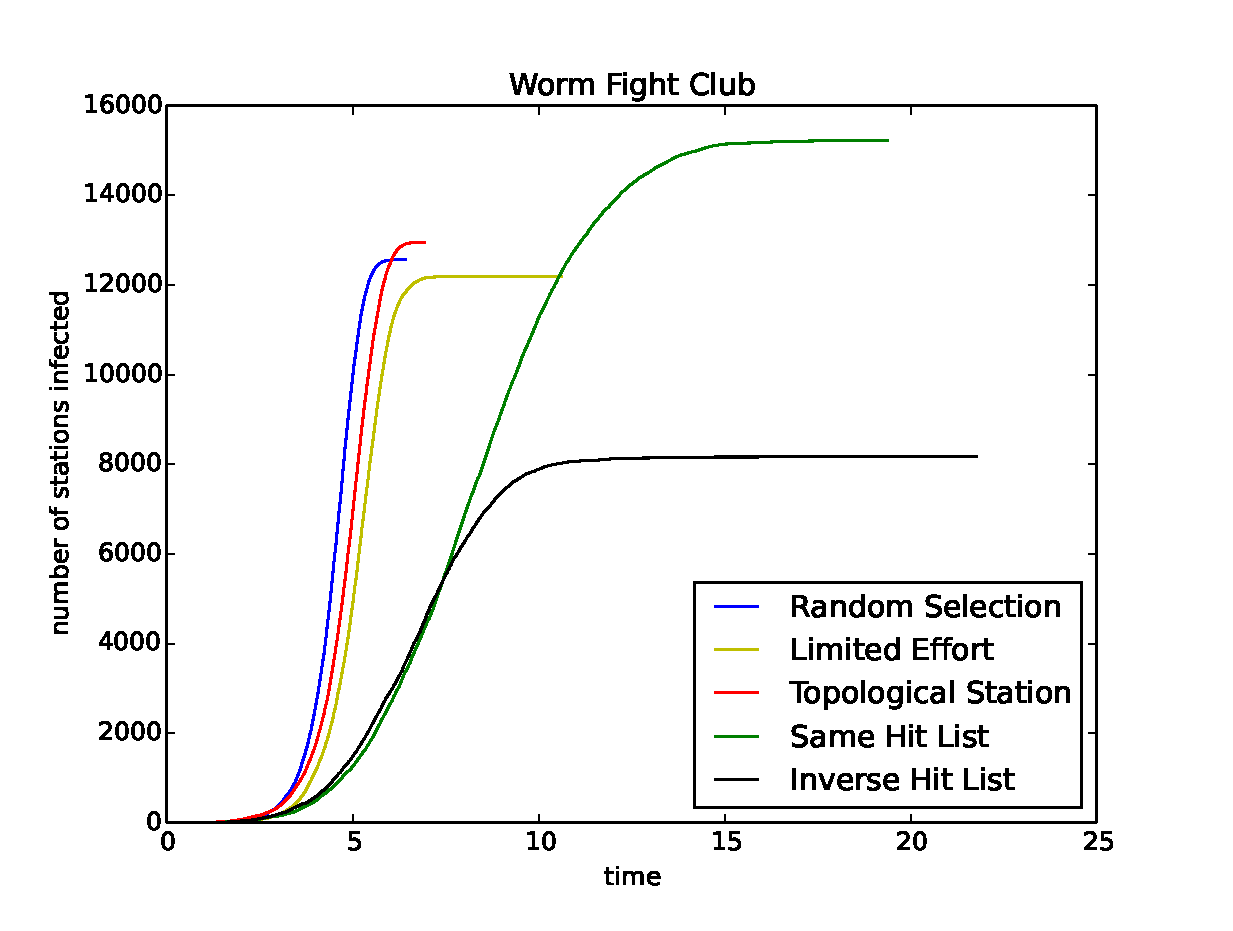
\includegraphics[width=0.8\textwidth]{figure6.1.eps}
\caption{Worm Fight Club: Bad worms v.s. Cheese worms}
\end{center}
\end{figure}

As you can see we have two curves for the "hit list worms fight". For the "Same Hit List" we mean that, with a hit list that defines all hosts within the class B address range, both the good worms and bad worms are starting the first station on the list (from lower station IDs to higher station IDs). While for the "Inverse Hit List", we let the bad worms act the same way, but let the good worms start to use the last station on the hit list (from higher station IDs to lower station IDs). 

Now, for the results, under the defense of cheese worm using the same selection method (except for the inverse cheese worm), the number of infected hosts are all less than the number of vulnerable machines ($254\times254\times0.25 = 16,129$), and the cheese worm using the inverse hit list only let the bad worms to achiever half of the total vulnerable machines. In terms of the time to infect all the available vulnerable machines (excluding the vulnerable hosts get patched by the cheese worms), worms using random selection method are still the fast, and the limited effort worms and topological station selection worms are not much slower than the random selection worms, while the worms using hit lists are still the slowest. 


\subsection*{6.2}

Here, our results are only based on random selection method, since this is the fastest worm that to infect all vulnerable machines, and we always let he bad worms to be contacted first. We still set the total vulnerable machines to be $254\times254\times0.25 =16,129$. 

\begin{table}[H]
\begin{center}
\begin{tabular}{| c || c | c | }
  \hline
$ Experiment $&$ Infected $&$Percentage(\%)$ 
\\  \hline
$1$&$ 12,563 $&$ 77.89  $
\\  \hline
$2$&$ 12,561 $&$ 77.87  $
\\  \hline
$3$&$ 12,551 $&$ 77.81  $
\\  \hline
$4$&$ 12,563 $&$ 77.89  $
\\  \hline
$5$&$ 12,560 $&$ 77.87  $
\\  \hline
$5$&$ 12,555 $&$ 77.84  $
\\  \hline
\end{tabular}
\end{center}
\caption{Experiments on Random Selection Worms}
\end{table}

The average of infected machines are $12,560$ and quite centralized, so I don't put bar chart here. This is what I am expected, under such a big B class space, when let the bad worms be contacted first, in the end, the ratio of the infected hosts should be convergent to some fixed point. 


%
%\begin{figure}[H]
%\begin{center}
%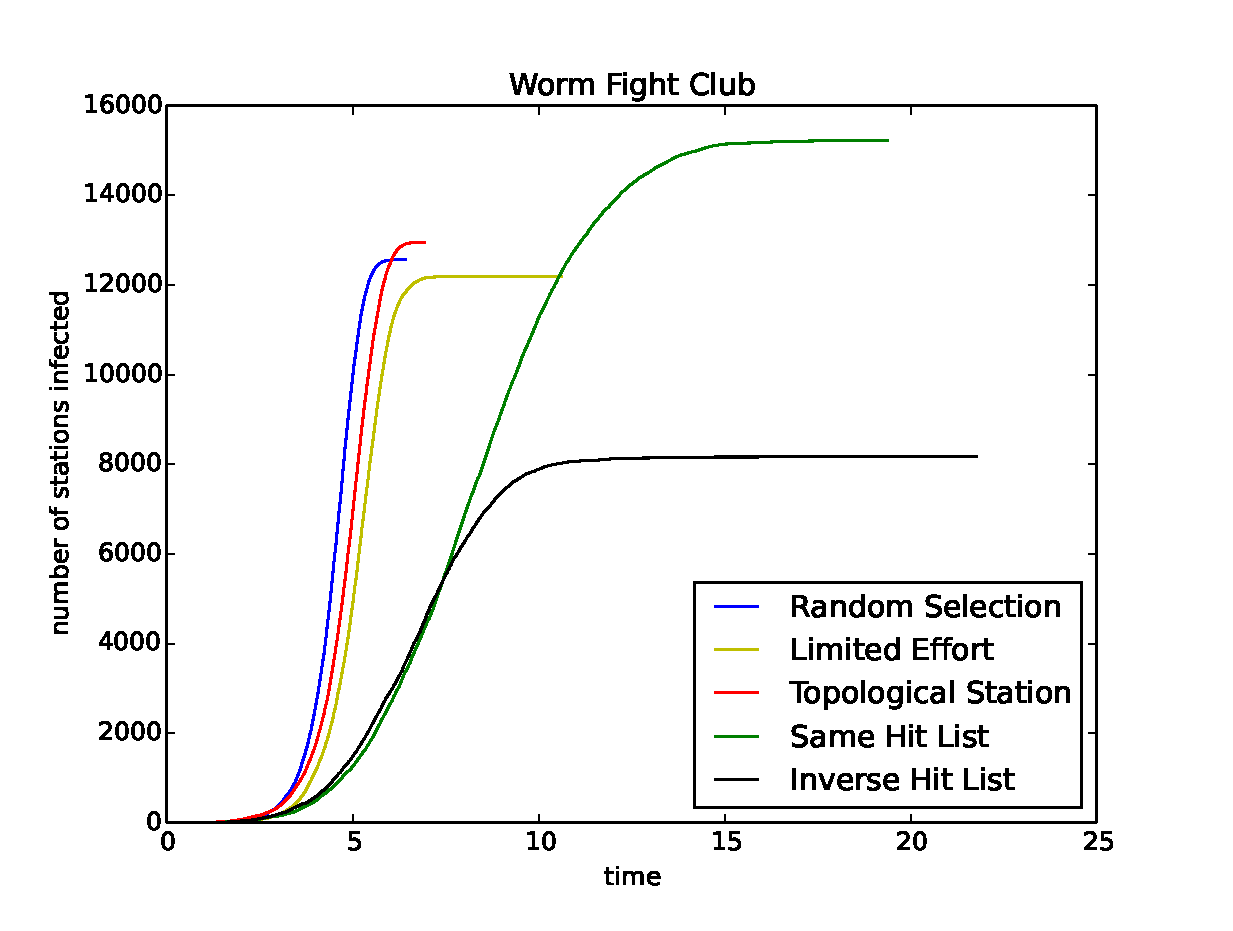
\includegraphics[width=0.8\textwidth]{figure6.1.eps}
%\caption{Worm Fight Club: the affection of Cheese worms}
%\end{center}
%\end{figure}







% \Section{Free Style}

% For this part of the project develop your own selection method.
% You method will be graded on novelty, speed, and infection
% attempts. The objectives are fast network infection and a low
% number of attempts per vulnerable machine. Assume 25\% of the
% stations are vulnerable.

% \Questions{20}
% You must also correctly answer the following questions to receive
% full credit for this part of the project.
% \begin{enumerate}
%   \item Describe how the worm randomly selects a station.

%   \item Plot the number of stations infected as time increases
% (use hours for time). Describe the performance of the station
% selection method.

%   \item Plot the time until initial infection per vulnerable
% station (3 dimensional plot). Describe the time required per
% station. Is the time the same for stations? What is the average
% and standard deviation infection time? Comment on your results.

%   \item Plot the number of infection attempts per vulnerable
% station (3 dimensional plot).Describe the time required per
% station. Is the number of infection attempts the same for
% stations? What is the average and standard deviation number of
% infection attempts? Comment on your results.

%   \item Change the vulnerable percentage to 50\% and repeat the
% first four questions. Is there a difference between the
% percentages? Why or why not?
% \end{enumerate}


\end{document}
